\documentclass{book}

\usepackage{amsmath}
\usepackage{fullpage}
\usepackage[colorlinks]{hyperref}
\usepackage{bm}
\usepackage{listings}
\usepackage{color}
\usepackage{graphicx}
\usepackage{natbib}
\usepackage{cancel}
\usepackage{amsthm}

\hypersetup{
    citecolor = {blue}
}

\title{Formulas relating to pulsars}
\author{Sam McSweeney}

\newcommand{\phase}{\varphi}
\newcommand{\deriv}[2]{\frac{\text{d}{#1}}{\text{d}{#2}}}
\newcommand{\derivn}[3]{\frac{\text{d}^{#3}{#1}}{\text{d}{#2}^{#3}}}
\newcommand{\pd}[2]{\frac{\partial {#1}}{\partial {#2}}}
\newcommand{\ppd}[2]{\frac{\partial^2{#1}}{\partial {#2}^2}}
\newcommand{\pdpd}[3]{\frac{\partial^2{#1}}{\partial {#2} \partial {#3}}}
\newcommand{\F}[1]{\bm{F}_{#1}}
\newcommand{\ph}{\phi_\ast}
\newcommand{\unitvec}[1]{\hat{\bm{#1}}}
\newcommand{\shat}{\hat{\bf s}}

\newcommand{\linktosage}[1]{\hyperref[#1]{[Sage script]}}

\definecolor{mygreen}{rgb}{0,0.6,0}

\lstset{
    basicstyle=\footnotesize\ttfamily,
    frame=single,
    language=Python,
    breaklines=true,
    title=\lstname,
    keywordstyle=\color{mygreen}
}

\newtheorem{theorem}{Theorem}[section]
\newtheorem{lemma}[theorem]{Lemma}

\bibliographystyle{chicago}

\begin{document}

\maketitle

\tableofcontents

\chapter{Pulsars}

\section{Notation and definitions}

The ``viewing geometry'' refers to the angles $\alpha$ (the angle between the pulsar's rotation axis and its magnetic axis) and $\zeta$ (the angle between the rotation axis and the line of sight), both of which are assumed constant over observing timescales. When the pulsar is at some rotation phase $\phase$, the spherical triangle defined by the rotation axis ($\hat{\omega}$), the magnetic axis ($\hat{\mu}$), and the line of sight ($\hat{n}$) is shown in Fig \ref{fig:pulsarangles}. The common names for these angles are listed in Table \ref{tbl:pulsarangles}.

\begin{figure}[!ht]
    \centering
    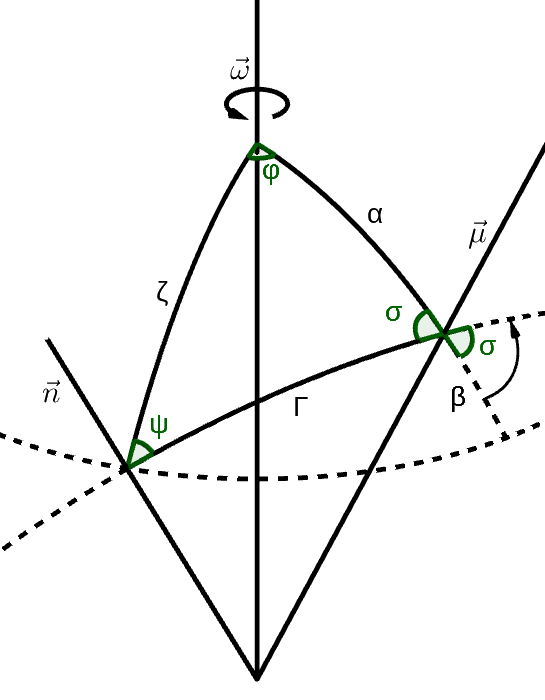
\includegraphics[scale=0.3]{images/pulsarangles.png}
    \caption{The spherical triangle defined by $\hat{\omega}$, $\hat{\mu}$, and $\hat{n}$. The common names of all the angles in the diagram are given in Table \ref{tbl:pulsarangles}.}
    \label{fig:pulsarangles}
\end{figure}

\begin{table}[!ht]
    \centering
    \caption{The fundamental triangle of the pulsar viewing geometry.}
    \label{tbl:pulsarangles}
    \begin{tabular}{c|l}
        \hline
        Angle & Common name \\
        \hline
        $\alpha$ & Inclination angle \\
        $\zeta$  & Observer angle \\
        $\beta$  & Impact angle \\
        $\Gamma$ & Beam opening angle \\
        $\phase$ & Rotation phase \\
        $\psi$   & Polarisation angle \\
        $\sigma$ & Magnetic azimuth \\
        \hline
    \end{tabular}
\end{table}

\subsection{Identities of the fundamental triangle}

From the spherical law of sines:
\begin{equation}
    \begin{aligned}
    \sin\zeta  &= \frac{\sin\Gamma \sin\sigma}{\sin\phase}
                = \frac{\sin\alpha \sin\sigma}{\sin\psi} &\qquad
    \sin\sigma &= \frac{\sin\phase \sin\zeta}{\sin\Gamma}
                = \frac{\sin\psi \sin\zeta}{\sin\alpha} \\
    \sin\alpha &= \frac{\sin\Gamma \sin\psi}{\sin\phase}
                = \frac{\sin\zeta \sin\psi}{\sin\sigma} &
    \sin\psi   &= \frac{\sin\sigma\sin\alpha}{\sin\zeta}
                = \frac{\sin\phase \sin\alpha}{\sin\Gamma} \\
    \sin\Gamma &= \frac{\sin\alpha \sin\phase}{\sin\psi}
                = \frac{\sin\zeta \sin\phase}{\sin\sigma} &
    \sin\phase &= \frac{\sin\sigma \sin\Gamma}{\sin\zeta}
                = \frac{\sin\psi \sin\Gamma}{\sin\alpha}
    \end{aligned}
\end{equation}
From the spherical law of cosines:
\begin{equation}
    \begin{aligned}
        \cos\zeta  &=  \cos\alpha \cos\Gamma + \sin\alpha \sin\Gamma \cos\sigma, &\qquad
        \cos\sigma &= -\cos\phase \cos\psi   + \sin\phase \sin\psi   \cos\zeta,  \\[5pt]
        \cos\alpha &=  \cos\zeta  \cos\Gamma + \sin\zeta  \sin\Gamma \cos\psi,   &
        \cos\psi   &= -\cos\phase \cos\sigma + \sin\phase \sin\sigma \cos\alpha, \\[5pt]
        \cos\Gamma &=  \cos\zeta  \cos\alpha + \sin\zeta  \sin\alpha \cos\phase, &
        \cos\phase &= -\cos\sigma \cos\psi   + \sin\sigma \sin\psi   \cos\Gamma
    \end{aligned}
\end{equation}
Each of the angles in terms of $\alpha$, $\zeta$, and $\phase$:
\begin{equation}
    \begin{aligned}
        \tan\psi   &= \frac{\sin\alpha \sin\phase}{\sin\zeta \cos\alpha - \cos\zeta \sin\alpha \cos\phase}, \\[5pt]
        \tan\sigma &= \frac{\sin\zeta  \sin\phase}{\sin\alpha \cos\zeta - \cos\alpha \sin\zeta \cos\phase}, \\[10pt]
        \cos\Gamma &= \cos\zeta  \cos\alpha + \sin\zeta  \sin\alpha \cos\phase
    \end{aligned}
\end{equation}
Other $\tan$ identities:
\begin{equation}
    \begin{aligned}
        \tan\alpha &= \frac{\sin\psi \sin\Gamma}{\sin\sigma \cos\psi + \cos\sigma \sin\psi \cos\Gamma}, \\[5pt]
        \tan\zeta  &= \frac{\sin\sigma \sin\Gamma}{\sin\psi \cos\sigma + \cos\psi \sin\sigma \cos\Gamma}
    \end{aligned}
\end{equation}
Holding $\alpha$ and $\zeta$ constant, we also have the rate of change with respect to $\phase$:
\begin{equation}
    \begin{aligned}
        \deriv{\psi}{\phase}
            &= -\frac{\sin\alpha \cos\sigma}{\sin\Gamma}
             = -\frac{\sin\psi \cos\sigma}{\sin\phase} \\[5pt]
        \deriv{\sigma}{\phase}
            &= -\frac{\sin\zeta \cos\psi}{\sin\Gamma}
             = -\frac{\sin\sigma \cos\psi}{\sin\phase} \\[5pt]
        \deriv{\Gamma}{\phase}
            &= \sin\alpha \sin\sigma
             = \sin\zeta  \sin\psi
    \end{aligned}
\end{equation}
A perhaps slightly more convenient formulation of the above (in order to avoid square roots and related sign ambiguities):
\begin{equation}
    \begin{aligned}
        \deriv{\psi}{\phase}
            &= -\frac{\sin\psi\cos\sigma}{\sin\phase}
             = -\frac{\tan\psi\cos^2\sigma}{\sin\phase}\frac{\cos\psi}{\cos\sigma}
             = \frac{\tan\psi}{1 + \tan^2\sigma}\bigg(\frac{1}{\tan\phase} - \tan\sigma\cos\alpha\bigg) \\
        \deriv{\sigma}{\phase}
            &= -\frac{\sin\sigma\cos\psi}{\sin\phase}
             = -\frac{\tan\sigma\cos^2\psi}{\sin\phase}\frac{\cos\sigma}{\cos\psi}
             = \frac{\tan\sigma}{1 + \tan^2\psi}\bigg(\frac{1}{\tan\phase} - \tan\psi\cos\zeta\bigg)
    \end{aligned}
\end{equation}
The following relations also hold:
\begin{equation}
    \begin{aligned}
        \deriv{\sigma}{\phase} + \deriv{\psi}{\phase}\cos\Gamma &= -\cos\alpha \\[5pt]
        \deriv{\sigma}{\phase}\cos\Gamma + \deriv{\psi}{\phase} &= -\cos\zeta \\[5pt]
        \left(\deriv{\sigma}{\phase}\right)^2 - \left(\deriv{\psi}{\phase}\right)^2
            &= -\deriv{\sigma}{\phase}\cos\alpha + \deriv{\psi}{\phase}\cos\zeta \\[5pt]
        \derivn{\sigma}{\phase}{2} &= -\frac{\sin\alpha\sin\zeta}{\sin^2\Gamma}(\sin\psi\cos\sigma - \sin\sigma\cos\psi\cos\Gamma)\\[5pt]
        \derivn{\psi}{\phase}{2} &= -\frac{\sin\alpha\sin\zeta}{\sin^2\Gamma}(\sin\sigma\cos\psi - \sin\psi\cos\sigma\cos\Gamma)
    \end{aligned}
\end{equation}
At the fiducial point ($\phase = 0^\circ$):
\begin{equation}
    \chi_0 \equiv \left.\deriv{\psi}{\phase}\right|_{\phase = 0^\circ}
        = -\frac{\sin\alpha}{\sin\zeta\cos\alpha - \cos\zeta\sin\alpha}
        = -\frac{\sin\alpha}{\sin(\zeta - \alpha)}
        \equiv -\frac{\sin\alpha}{\sin\beta}
\end{equation}
At the anti-fiducial point ($\phase = 180^\circ$):
\begin{equation}
    \chi_{180} \equiv \left.\deriv{\psi}{\phase}\right|_{\phase = 180^\circ}
        = \frac{\sin\alpha}{\sin\zeta\cos\alpha + \cos\zeta\sin\alpha}
        = \frac{\sin\alpha}{\sin(\zeta + \alpha)}
\end{equation}
Consequently,
\begin{equation}
    \cos\zeta = -\frac{1}{2}\left(\frac{1}{\chi_0} + \frac{1}{\chi_{180}}\right)
\end{equation}

\subsection{Example derivations}

Here is a derivation for the identity
\begin{equation}
    \deriv{\sigma}{\phase} = -\frac{\sin\sigma \cos\psi}{\sin\phase}.
\end{equation}
Starting with
\begin{equation}
    \tan\sigma = \frac{\sin\zeta \sin\phase}{\sin\alpha \cos\zeta - \cos\alpha \sin\zeta \cos\phase},
\end{equation}
implicit differentiation with respect to $\phase$ (and remembering that $\alpha$ and $\zeta$ are constant) yields:
\begin{equation}
    \begin{aligned}
    \frac{1}{\cos^2\sigma} \deriv{\sigma}{\phase}
        &= \frac{\sin\zeta \cos\phase}{\sin\alpha \cos\zeta - \cos\alpha \sin\zeta \cos\phase} -
            \frac{\sin\zeta \sin\phase}{(\sin\alpha \cos\zeta - \cos\alpha \sin\zeta \cos\phase)^2} \cdot (\cos\alpha \sin\zeta \sin\phase) \\
        &= \frac{\sin\zeta \cos\phase (\sin\alpha \cos\zeta - \cos\alpha \sin\zeta \cos\phase) -
            \sin\zeta \sin\phase \cos\alpha \sin\zeta \sin\phase}{(\sin\alpha \cos\zeta - \cos\alpha \sin\zeta \cos\phase)^2} \\
        &= \frac{\sin\zeta \cos\zeta \sin\alpha \cos\phase - \sin^2\zeta \cos\alpha}{(\sin\alpha \cos\zeta - \cos\alpha \sin\zeta \cos\phase)^2} \\
        &= \frac{\tan^2\sigma (\sin\zeta \cos\zeta \sin\alpha \cos\phase - \sin^2\zeta \cos\alpha)}{\sin^2\zeta \sin^2\phase} \\
    \end{aligned}
\end{equation}
Then,
\begin{equation}
    \begin{aligned}
    \deriv{\sigma}{\phase}
        &= \frac{\sin^2\sigma (\cos\zeta \sin\alpha \cos\phase - \sin\zeta \cos\alpha)}{\sin\zeta \sin^2\phase} \\
        &= -\frac{\sin^2\sigma \sin\alpha \sin\phase}{\sin\zeta \sin^2\phase \tan\psi} \\
        &= -\frac{\sin^2\sigma \sin\alpha}{\sin\zeta \sin\phase \tan\psi} \\
        &= -\frac{\sin^2\sigma \cos\psi}{\sin\phase} \frac{\sin\alpha}{\sin\zeta \sin\psi} \\
        &= -\frac{\sin^2\sigma \cos\psi}{\sin\phase} \frac{1}{\sin\sigma} \\
        &= -\frac{\sin\sigma \cos\psi}{\sin\phase}
    \end{aligned}
\end{equation}

\section{Magnetic Vector Field}

\subsection{Dipole}

\subsubsection{Coordinate-free expression}

The magnetic field, in coordinate-free notation, centred at the origin \linktosage{sage:Bdip}:
\begin{equation}
    \begin{aligned}
        \bm{B}(\bm{r})
            &= B_0\left(\frac{r_0}{r}\right)^3\frac{3(\unitvec{\mu}\cdot\unitvec{r})\unitvec{r} - \unitvec{\mu}}{2} \\
            &= B_0\left(\frac{r_0}{r}\right)^3\frac{3\cos\theta\,\unitvec{r} - \unitvec{\mu}}{2},
    \end{aligned}
\end{equation}
where $B_0$ is the magnetic field strength at the poles at distance $r_0$ from the origin.
Its magnitude is:
\begin{equation}
\begin{aligned}
    B({\bm{r}}) = |\bm{B}(\bm{r})|
        &= B_0\left(\frac{r_0}{r}\right)^3 \frac{\sqrt{(3\cos\theta\,\unitvec{r} - \unitvec{\mu}) \cdot (3\cos\theta\,\unitvec{r} - \unitvec{\mu}) }}{2} \\
        &= B_0\left(\frac{r_0}{r}\right)^3 \frac{\sqrt{ 9\cos^2\theta\,\unitvec{r}\cdot\unitvec{r} - 6\cos\theta\,\unitvec{r}\cdot\unitvec{\mu} + \unitvec{\mu}\cdot\unitvec{\mu} }}{2} \\
        &= B_0\left(\frac{r_0}{r}\right)^3 \frac{\sqrt{ 9\cos^2\theta - 6\cos^2\theta + 1 }}{2} \\
        &= B_0\left(\frac{r_0}{r}\right)^3 \frac{\sqrt{3\cos^2\theta + 1}}{2}
\end{aligned}
\end{equation}
and the normalised field is:
\begin{equation}
    \unitvec{B}(\bm{r})
        = \frac{\bm{B}(\bm{r})}{B(\bm{r})}
        = \frac{3\cos\theta \, \unitvec{r} - \unitvec{\mu}}{\sqrt{3\cos^2\theta + 1}}
\end{equation}

\subsubsection{Cartesian coordinates}

When the magnetic dipole is aligned with the $z$-axis (i.e. $\unitvec{\mu} = \unitvec{z}$), in Cartesian coordinates (but still using the shorthand $r = \sqrt{x^2 + y^2 + z^2}$) \linktosage{sage:Bdip_aligned}:
\begin{equation}
\begin{aligned}
    \bm{B}(\bm{r})
        &= B_0\left(\frac{r_0}{r}\right)^3\frac{3\cos\theta\,\unitvec{r} - \unitvec{\mu}}{2} \\
        &= B_0\left(\frac{r_0}{r}\right)^3\frac{3r\cos\theta (x\unitvec{x} + y\unitvec{y} + z\unitvec{z}) - r^2\unitvec{z}}{2r^2} \\
        &= B_0\left(\frac{r_0}{r}\right)^3\frac{3z(x\unitvec{x} + y\unitvec{y} + z\unitvec{z}) - r^2\unitvec{z}}{2r^2} \\
        &= B_0\left(\frac{r_0}{r}\right)^3\frac{3xz\,\unitvec{x} + 3yz\,\unitvec{y} + (3z^2 - r^2)\,\unitvec{z}}{2r^2}
\end{aligned}
\end{equation}
Or, if you define the reduced quantities:
\begin{align}
    x_r &\equiv \frac{x}{r} = \cos\phi\sin\theta, &
    y_r &\equiv \frac{y}{r} = \sin\phi\sin\theta, &
    z_r &\equiv \frac{z}{r} = \cos\theta,
\end{align}
then it can also be written
\begin{equation}
    \bm{B}(\bm{r})
        = B_0\left(\frac{r_0}{r}\right)^3\frac{3 x_r z_r \,\unitvec{x} + 3 y_r z_r \,\unitvec{y} + (3 z_r^2 - 1)\,\unitvec{z}}{2}.
\end{equation}
The corresponding normalised magnetic field is
\begin{equation}
\begin{aligned}
    \unitvec{B}(\vec{r})
        &= \frac{3xz\,\unitvec{x} + 3yz\,\unitvec{y} + (3z^2 - r^2)\,\unitvec{z}}{r^2\sqrt{3\cos^2\theta + 1}} \\
        &= \frac{3xz\,\unitvec{x} + 3yz\,\unitvec{y} + (3z^2 - r^2)\,\unitvec{z}}{r\sqrt{3z^2 + r^2}} \\
        &= \frac{3 x_r z_r \, \unitvec{x} + 3 y_r z_r \,\unitvec{y} + (3 z_r^2 - 1)\,\unitvec{z}}{\sqrt{3z_r^2 + 1}}
\end{aligned}
\end{equation}
When the magnetic dipole is tilted in the $xz$-plane by angle $\alpha$ \linktosage{sage:Bdip_inclined}:
\begin{equation}
    \bm{B}(\bm{r}) =
    \frac{\mu\cos\alpha}{r^5}\begin{bmatrix}
        3xz \\
        3yz \\
        3z^2 - r^2
    \end{bmatrix} + 
    \frac{\mu\sin\alpha}{r^5}\begin{bmatrix}
        3x^2 - r^2 \\
        3xy \\
        3xz
    \end{bmatrix}
\end{equation}

\subsubsection{Spherical coordinates}

To translate from Cartesian to spherical, we need the identity $\unitvec{z} = \cos\theta \,\unitvec{r} - \sin\theta\,\unitvec{\theta}$.
For the aligned case ($\unitvec{\mu} = \unitvec{z}$),
\begin{equation}
\begin{aligned}
    \bm{B}(\bm{r})
        &= B_0\left(\frac{r_0}{r}\right)^3\frac{3\cos\theta\,\unitvec{r} - \unitvec{\mu}}{2} \\
        &= B_0\left(\frac{r_0}{r}\right)^3\frac{3\cos\theta\,\unitvec{r} - \cos\theta \,\unitvec{r} + \sin\theta\,\unitvec{\theta}}{2} \\
        &= B_0\left(\frac{r_0}{r}\right)^3\left(\cos\theta\,\unitvec{r} + \frac12 \sin\theta\,\unitvec{\theta}\right),
\end{aligned}
\end{equation}
which is the form given in Eq. (1) of \citet{Davis1947}, except for a difference in sign.

\subsection{Deutsch-Arendt equations}

\begin{equation}
\begin{aligned}
    \vec{B}(\vec{r}) &= \mu \cos{\alpha} \F{1} \frac{1}{r^5} + \\
                   &\hspace{13pt} \mu \sin{\alpha} \F{2} \frac{\cos(\ph)}{r^3 r_L^2} +
                                  \mu \sin{\alpha} \F{3} \bigg(\frac{\cos(\ph)}{r^5} + \frac{\sin(\ph)}{r^4 r_L}\bigg) - \\
                   &\hspace{13pt} \mu \sin{\alpha} \F{4} \frac{\sin(\ph)}{r^3 r_L^2} -
                                  \mu \sin{\alpha} \F{5} \bigg(\frac{\sin(\ph)}{r^5} - \frac{\cos(\ph)}{r^4 r_L}\bigg)
\end{aligned}
\end{equation}
where
\begin{equation}
\begin{aligned}
    \F{1} &= 3xz\,\hat{x} + 3yz\,\hat{y} + (3z^2-r^2)\,\hat{z} \\
    \F{2} &= (r^2-x^2)\,\hat{x} - xy\,\hat{y} - xz\,\hat{z} \\
    \F{3} &= (3x^2-r^2)\,\hat{x} + 3xy\,\hat{y} + 3xz\,\hat{z} \\
    \F{4} &= -xy\,\hat{x} + (r^2-y^2)\,\hat{y} - yz\,\hat{z} \\
    \F{5} &= 3xy\,\hat{x} + (3y^2-r^2)\,\hat{y} + 3yz\,\hat{z}
\end{aligned}
\end{equation}
and
\begin{equation}
    \ph = \frac{r - r_p}{r_L}
\end{equation}


\section{Field Lines}

Consider a single field line in a plane, whose coordinates are chosen (without loss of generality) so that the magnetic moment is aligned with the $z$-axis.
Also, let distances be normalised to some characteristic length, $r_L$, so that $r^\prime = r/r_L$.
Let the maximum distance of the field line from the origin be $R^\prime = R/r_L$.
One can write down the equation for the line in either Cartesian or polar coordinates.
The relations between the various coordinates are found in Table \ref{tbl:dipolar}.
\begin{table}[!ht]
    \centering
    \caption{Each coordinate in terms of the others}
    \label{tbl:dipolar}
    \begin{tabular}{c|cccc}
        & $r$ & $\theta$ & $x$ & $z$ \\[5pt]
        \hline
        $r^\prime =$ & --- & $R^\prime\sin^2\theta$ & $\sqrt[3]{R^\prime (x^\prime)^2}$ & ? \\[8pt]
        $\theta =$   & $\sin^{-1}\sqrt{\dfrac{r^\prime}{R^\prime}}$ & --- & $\sin^{-1}\sqrt[3]{\dfrac{x^\prime}{R^\prime}}$ & ? \\[8pt]
        $x^\prime =$ & $r^\prime\sqrt{\dfrac{r^\prime}{R^\prime}}$ & $R^\prime\sin^3\theta$ & --- & (see below) \\[8pt]
        $z^\prime =$ & $r^\prime\sqrt{1-\dfrac{r^\prime}{R^\prime}}$ & $R^\prime\sin^2\theta\cos\theta$ & $(x^\prime)^{2/3} \sqrt{(R^\prime)^{2/3} - (x^\prime)^{2/3}}$ & ---
    \end{tabular}
\end{table}

Getting the formulas in terms of $z$ involves solving high-order polynomial equations.
For instance, points on the line characterised by $R^\prime$ satisfy:
\begin{equation}
    0 = x^6 + (3z^2 - R^2)x^4 + 3z^4x^2 + z^6,
\end{equation}
where I have omitted the primes for brevity.
The roots (in $x$) are expressible as closed-form functions of $R$ and $z$, but I do not them include here.
The formulas for the other variables can be found similarly.

\subsection{Derivatives}

See Table \ref{tbl:dipolarderiv}.
We use the definition $d\ell = \sqrt{dx^2+dz^2}$.

\begin{table}[!p]
    \centering
    \caption{The derivatives of the expressions in Table \ref{tbl:dipolar}}
    \label{tbl:dipolarderiv}
    \begin{tabular}{c|cccc}
        & $r$ & $\theta$ & $x$ & $z$ \\[5pt]
        \hline
        $dr/d\theta =$ & $2\sqrt{r(R-r)}$ & $2R\sin\theta\cos\theta$ & $2R^{1/3}x^{1/3}\sqrt{R^{2/3}-x^{2/3}}$ & ? \\[8pt]
        $dr/dx =$      & $\dfrac23\sqrt{\dfrac{R}{r}}$ & $\dfrac{2}{3\sin\theta}$ & $\dfrac23\sqrt[3]{\dfrac{R}{x}}$ & \\[8pt]
        $dr/dz =$      & & & & \\[8pt]
        \hline
        $d\theta/dr =$ & & & & \\[8pt]
        $d\theta/dx =$ & & & & \\[8pt]
        $d\theta/dz =$ & & & & \\[8pt]
        \hline
        $dx/dr =$      & $\dfrac32\sqrt{\dfrac{r}{R}}$ & & & \\[8pt]
        $dx/d\theta =$ & & $3R\sin^2\theta\cos\theta$ & $3x^{2/3} \sqrt{R^{2/3} - x^{2/3}}$ & $3z$ \\[8pt]
        $dx/dz =$      & & $\dfrac{3\sin\theta\cos\theta}{3\cos^2\theta-1}$ & $\dfrac{3x^{1/3}\sqrt{R^{2/3} - x^{2/3}}}{2R^{2/3} - 3x^{2/3}}$ & \\[8pt]
        \hline
        $dz/dr =$      & $\dfrac{2R-3r}{2\sqrt{R(R-r)}}$ & & & \\[8pt]
        $dz/d\theta =$ & $\sqrt{\dfrac{r}{R}}\left(2R-3r\right)$ & $R\sin\theta(3\cos^2\theta - 1)$ & $x^{1/3}(2R^{2/3} - 3x^{2/3})$ & \\[8pt]
        $dz/dx =$      & & $\dfrac{3\cos^2\theta-1}{3\sin\theta\cos\theta}$ & $\dfrac{2R^{2/3} - 3x^{2/3}}{3x^{1/3}\sqrt{R^{2/3} - x^{2/3}}}$ & \\[8pt]
        \hline
        $d\ell/dr =$ & $\dfrac12 \sqrt{\dfrac{4R-3r}{R-r}}$ & & & \\[8pt]
        $d\ell/d\theta =$ & & $R\sin\theta \sqrt{3\cos^2\theta + 1}$ & &
    \end{tabular}
\end{table}

\subsection{Arc Length}
The arc length of a field line, as a function of $\theta$:
\begin{equation}
    \begin{aligned}
        \int\,d\ell = \int\deriv{\ell}{\theta}\,d\theta
            &= \int R\sin\theta \sqrt{3\cos^2\theta + 1} \, d\theta \\
            &= -\frac{R}{6}\left(3\cos\theta\sqrt{3\cos^2\theta + 1} + \sqrt{3}\sinh^{-1}(\sqrt{3}\cos\theta)\right) + C
    \end{aligned}
\end{equation}
In particular, the arc length as measured from the origin is
\begin{equation}
    \ell_0(\theta) = -\frac{R}{6}\left(3\cos\theta\sqrt{3\cos^2\theta + 1} + \sqrt{3}\sinh^{-1}(\sqrt{3}\cos\theta)\right) +
                      \frac{R\sqrt{3}\sinh^{-1}\sqrt{3}}{6} + R
\end{equation}
whose Taylor expansion about $\theta = 0$ gives
\begin{equation}
    \frac{\ell_0}{R} \approx \theta^2 - \frac{13}{48}\theta^4 + \frac{241}{5760}\theta^6 + O(\theta^8)
    \label{eqn:arclengthth}
\end{equation}
The arc length, $\ell$, as a function of $r$:
\begin{equation}
    \begin{aligned}
        \ell = \int\,d\ell = \int\deriv{\ell}{r}\,dr
            &= \int \frac12 \sqrt{\frac{4R-3r}{R-r}} \, dr \\
            &= \frac{R}{12}\left(\frac{6S}{3 - S^2} + \sqrt{3}\log\left(\frac{S - \sqrt{3}}{S + \sqrt{3}}\right)\right) + C
    \end{aligned}
\end{equation}
where
\begin{equation}
    S = \sqrt{\frac{4R-3r}{R-r}}
\end{equation}
In particular, the arc length as measured from the origin is
\begin{equation}
    \ell_0 = \int_0^r \deriv{s}{r^\prime} \,dr^\prime
           = \frac{R}{12}\left(\frac{6S}{3 - S^2} + \sqrt{3}\log\left(\frac{S - \sqrt{3}}{S + \sqrt{3}}\right)\right) +
             R - \frac{R\sqrt{3}}{12}\log\left(\frac{2-\sqrt{3}}{2+\sqrt{3}}\right)
\end{equation}
and the arc length as measured from the surface is
\begin{equation}
    \begin{aligned}
        \ell_\text{surface} &= \int_{r_p}^r \deriv{s}{r^\prime} \,dr^\prime \\
               &= \frac{R}{12}\left(\frac{6S}{3 - S^2} + \sqrt{3}\log\left(\frac{S - \sqrt{3}}{S + \sqrt{3}}\right)\right) -
                  \frac{R}{12}\left(\frac{6S_{r_p}}{3 - S_{r_p}^2} + \sqrt{3}\log\left(\frac{S_{r_p} -
                  \sqrt{3}}{S_{r_p} + \sqrt{3}}\right)\right)
     \end{aligned}
\end{equation}
where
\begin{equation}
    S_{r_p} = \sqrt{\frac{4R-3r_p}{R-r_p}}
\end{equation}
A Taylor series expansion of $\ell_0$ about $r=0$ gives
\begin{equation}
    \ell_0 \approx r + \frac{r^2}{16R} + \frac{5r^3}{128R^2} + \frac{113r^4}{4096R^3} + O(r^5)
\end{equation}
in agreement with Eq \eqref{eqn:arclengthth} above.

\section{Footpoints}
\label{sec:footpoints}

Let $r_p$ be the pulsar's radius, and $\theta_p$ by the angle the footpoint makes with the magnetic axis.
\begin{align}
    r_p^\prime &= R^\prime\sin^2\theta_p \\
    \theta_p &= \sin^{-1}\sqrt{\frac{r_p^\prime}{R^\prime}} = \sin^{-1}\sqrt{\frac{r_p^\prime\sin^2\theta}{r^\prime}} \\
    \theta   &= \sin^{-1}\left[\sqrt{\frac{r^\prime}{r_p^\prime}}\sin\theta_p\right] \label{eqn:thp_to_th}
\end{align}
To normalise a footpoint with respect to the footpoint of the last open field lines ($R = r_L \equiv \frac{cP}{2\pi}$), we define
\begin{equation}
    \theta_L \equiv \sin^{-1}\sqrt{r_p^\prime}
\end{equation}
and then
\begin{equation}
    s \equiv \frac{\theta_p}{\theta_L}
\end{equation}
To convert from a given $s$ to $R$:
\begin{equation}
    R^\prime = \frac{r_p^\prime}{\sin^2\left(s\sin^{-1}\sqrt{r_p^\prime}\right)}
\end{equation}
Given the $s$ and $r$ of an arbitrary point in the magnetosphere, the point's colatitude is
\begin{equation}
    \theta = \sin^{-1}\sqrt{\frac{r^\prime}{r_p^\prime}\sin^2\left(s \sin^{-1}\sqrt{r_p^\prime}\right)}
\end{equation}
and its height is
\begin{equation}
    \begin{aligned}
        r^\prime &= \frac{r_p^\prime\sin^2\theta}{\sin^2\left(s \sin^{-1}\sqrt{r_p^\prime}\right)} \\
        \frac{r^\prime}{\sin^2\theta} = R^\prime &\approx \frac{1}{s^2} - \frac{r_p^\prime}{3s^2} + O\left[(r_p^\prime)^2\right]
    \end{aligned}
\end{equation}
where the Taylor expansion was taken about $r_p^\prime = 0$.
Its partial derivative with respect to $s$ is
\begin{equation}
    \begin{aligned}
        \pd{r^\prime}{s} &= -\frac{2r_p^\prime \cos\left(s\,\sin^{-1}\sqrt{r_p^\prime}\right) \sin^{-1}\sqrt{r_p^\prime} \sin^2\theta}{
                                   \sin^3\left(s\,\sin^{-1}\sqrt{r_p^\prime}\right)} \\
        \frac{1}{\sin^2\theta} \pd{r^\prime}{s} &\approx -\frac{2}{s^3} + \frac{2r_p^\prime}{3s^3} + O\left[\left(r_p^\prime\right)^2\right]
    \end{aligned}
\end{equation}

\section{Curvature}

\subsection{Aligned rotator, without rotation effects}
From Eq \eqref{eqn:curvature_polar},
\begin{equation}
    \begin{aligned}
        \kappa^\prime &= \frac{3\sin\theta(\cos^2\theta + 1)}{r^\prime(3\cos^2\theta + 1)^{3/2}} \\
        \rho^\prime = \frac{1}{\kappa^\prime}
            &= \frac{r^\prime(3\cos^2\theta + 1)^{3/2}}{3\sin\theta(\cos^2\theta + 1)}
    \end{aligned}
\end{equation}
\citet{Gangadhara2004} gives it in this form (see their Eq. (4)):
\begin{equation}
    \rho = \frac{R\sin\theta(5 + 3\cos(2\theta))^{3/2}}{3\sqrt{2}(3 + \cos(2\theta))}
\end{equation}
Taylor expansions about $\theta = 0$:
\begin{equation}
    \begin{aligned}
        \kappa^\prime r^\prime &\approx \frac34 \theta + \frac{11}{32} \theta^3 + \frac{361}{2560} \theta^5 + O(\theta^7) \\
        \frac{\rho^\prime}{r^\prime} &\approx \frac43 \theta^{-1} - \frac{11}{18}\theta + \frac{127}{4320}\theta^3 + O(\theta^5)
    \end{aligned}
\end{equation}
\begin{figure}[!p]
    \centering
    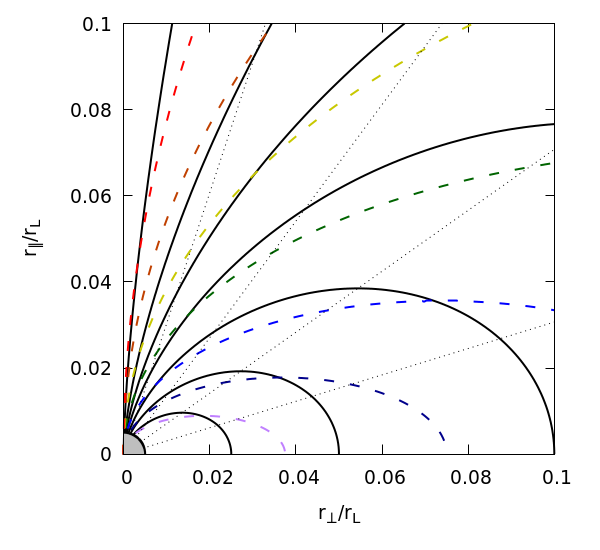
\includegraphics[scale=0.45]{images/curvature-no-rotation.png}
    \caption{Lines of constant curvature (dashed, coloured), neglecting rotation effects on particle trajectory curvature. Red to purple colours run from small to large curvatures $\kappa$ (and hence, from low to high frequencies, assuming a constant $\gamma$ value). The solid black lines are the dipole field lines, and the dotted black lines are the lines of constant tangent.}
    \label{fig:curvature-no-rotation}
\end{figure}

\subsection{Aligned rotator, with rotation effects}
\begin{equation}
    \begin{aligned}
        \kappa^\prime &= \frac{\sqrt{3}\sin\theta(12\cos^8\theta + 96\cos^6\theta + 71\cos^4\theta + 14\cos^2\theta + 1)^{1/2}}{
                               r^\prime(3\cos^2\theta+1)^{3/2}} \\
                           \rho^\prime   &= \frac{r^\prime(3\cos^2\theta+1)^{3/2}}{
                               \sqrt{3}\sin\theta(12\cos^8\theta + 96\cos^6\theta + 71\cos^4\theta + 14\cos^2\theta + 1)^{1/2}}
    \end{aligned}
\end{equation}
A Taylor expansion about $\theta = 0$ gives
\begin{equation}
    \begin{aligned}
        \kappa^\prime &\approx \frac{3\sqrt{4(r^\prime)^2+1}}{4r^\prime}\,\theta -
                            \frac{52(r^\prime)^2 - 11}{32r^\prime\sqrt{4(r^\prime)^2+1}}\,\theta^3 +
                            O(\theta^5) \\
        \rho^\prime &\approx \frac{4r^\prime}{3\sqrt{4(r^\prime)^2+1}}\,\theta^{-1} +
                          \frac{r^\prime(52(r^\prime)^2 - 11)}{18(4(r^\prime)^2+1)^{3/2}}\,\theta +
                          O(\theta^3)
    \end{aligned}
\end{equation}
\begin{figure}[!p]
    \centering
    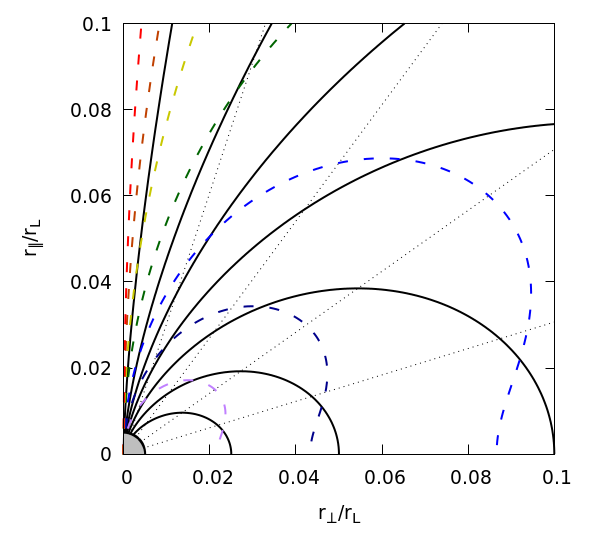
\includegraphics[scale=0.45]{images/curvature-with-rotation.png}
    \caption{Same as Fig. \ref{fig:curvature-no-rotation}, but including rotation effects (for an aligned rotator). The colours correspond to the same respective curvatures as in Fig. \ref{fig:curvature-no-rotation}.}
    \label{fig:curvature-with-rotation}
\end{figure}

\subsection{Inclined rotator \linktosage{sage:curvature}}

The Taylor expansion of the curvature near the magnetic axis ($\theta = 0$)
\begin{equation}
    \kappa^\prime \approx \frac{\sin\alpha}{\beta}\sqrt{4 + \left(\frac{r^\prime\cos\alpha}{\beta}\right)^2} + \dots
\end{equation}
Expanding around both $r = 0$ and $\theta = 0$:
\begin{equation}
   \kappa^\prime \approx 2\sin\alpha + 0r^\prime + ?\theta
\end{equation}
Note that this is in agreement with the expression ($\rho \approx r_L/(2\sin\alpha)$) stated in \citet{Thomas2007}.

\section{Beam Opening Angles}
\label{sec:beamopeningangles}

Let $\Gamma = \cos^{-1}(\hat{V}\cdot\hat{\mu})$ be the (half) opening angle of the beam.

\subsection{Beaming fraction}

The beaming fraction is the fractional area of the spherical cap with angular radius $\Gamma$,
\begin{equation}
    \frac{2\pi(1 - \cos\Gamma)}{4\pi}
        = \frac12 (1 - \cos\Gamma)
        = \sin^2\left(\frac{\Gamma}{2}\right).
\end{equation}

\subsection{Aligned rotator, without rotation effects}
The relationship between $\theta$ and $\Gamma$ (and its inverse) is given by \citet{Gangadhara2004}
\begin{equation}
    \begin{aligned}
        \cos(2\theta) &= \frac13\left(\cos\Gamma\sqrt{8 + \cos^2\Gamma} - \sin^2\Gamma\right) \\
        \sin^2\theta  &= -\frac16\left(\cos\Gamma\sqrt{8 + \cos^2\Gamma} + \cos^2\Gamma - 4\right) \\
        \tan\Gamma &= \frac{3\sin\theta\cos\theta}{3\cos^2\theta - 1}
    \end{aligned}
\end{equation}
Taylor series expansions (about $\theta = 0$ or $\Gamma = 0$):
\begin{equation}
    \begin{aligned}
        \theta &\approx \frac23 \Gamma - \frac2{81} \Gamma^3 + O(\Gamma^7) \\
        \sin^2\theta &\approx \frac{484}{729} - \frac{112}{243}\cos\Gamma - \frac{44}{243}\cos^2\Gamma + O(\cos^3\Gamma) \\
        \Gamma &\approx \frac32 \theta + \frac18 \theta^3 + \frac1{32} \theta^5 + O(\theta^7)
    \end{aligned}
\end{equation}

\subsection{Aligned rotator, with rotation effects}
\begin{equation}
    \cos\Gamma = \frac{\Lambda_\theta(3\cos^2\theta-1)}{\sqrt{3\cos^2\theta+1}}
\end{equation}
where
\begin{equation}
    \Lambda_\theta = \sqrt{1 - (r^\prime\sin\theta)^2}
\end{equation}
Taylor series expansions (about $\theta = 0$):
\begin{equation}
    \begin{aligned}
        \cos\Gamma &\approx 1 - \frac{4(r^\prime)^2+9}{8}\,\theta^2 -
                            \frac{48(r^\prime)^4 - 280(r^\prime)^2 - 9}{384}\,\theta^4 + O(\theta^6) \\
        \Gamma &\approx \sqrt{(r^\prime)^2 + \frac94}\,\theta +
                        \frac{8(r^\prime)^4 - 26(r^\prime)^2 + 9}{48\sqrt{(r^\prime)^2 + \frac94}}\,\theta^3 + O(\theta^5)
    \end{aligned}
\end{equation}

\subsection{Inclined rotator, with rotation effects \linktosage{sage:Gamma}}

The Taylor expansion of $\Gamma$ about $\theta = 0$ (in the magnetic frame) is
\begin{equation}
    \begin{aligned}
        \cos\Gamma &\approx \Lambda - r^\prime\sin\alpha
            \left(\frac{r^\prime\cos\alpha}{\Lambda}\cos\sigma +
                  \frac32\sin\sigma\right)\sin\theta + O(\sin^2\theta) \\
        \sin\Gamma &\approx r^\prime\sin\alpha +
            \left(r^\prime\cos\alpha\cos\sigma + \frac{3\Lambda}{2}\sin\sigma\right)\sin\theta +
            O(\sin^2\theta)
    \end{aligned}
\end{equation}
where
\begin{equation}
    \Lambda \equiv \sqrt{1-(r^\prime\sin\alpha)^2}
\end{equation}
Taylor expanding about both $r = 0$ and $\theta = 0$ gives:
\begin{equation}
    \begin{aligned}
        \cos\Gamma &\approx 1 - \frac12(r^\prime\sin\alpha)^2 -
            \frac32\theta r^\prime\sin\alpha\sin\sigma -
            \frac98\theta^2 - (r^\prime)^2\theta\sin\alpha\cos\alpha\cos\sigma +
            O(\text{4th order terms in $r$ and $\theta$}) \\
        \sin\Gamma &\stackrel{?}{\approx} r^\prime\sin\alpha + \frac32\theta\sin\sigma + r^\prime\cos\alpha\cos\sigma + \dots
    \end{aligned}
\end{equation}

\section{Characteristic age}

\citep[This same derivation is given briefly in][\S3.2.2.]{Lorimer2005}
Assume that the pulsar spindown is well described by
\begin{equation}
    \dot{\nu} = -K\nu^n,
\end{equation}
for some constants $K$ and $n$.
Expressing this in terms of the period ($\nu = 1/P$), we have
\begin{equation}
    \begin{aligned}
        \dot{\nu} = -\frac{\dot{P}}{P^2}
            &= -\frac{K}{P^n} \\
        \dot{P} &= KP^{2-n}.
    \end{aligned}
\end{equation}
This differential equation can be directly integrated by separation of variables.
We will assume $n \ne 1$ (to avoid an edge case), and also use $P_0$ for the initial period, $P$ for the current period, $P^\prime$ for the dummy variable under the integration, and $T$ for the age of the pulsar.
Then, integrating over the entire lifetime of the pulsar,
\begin{equation}
    \begin{aligned}
        \int_{P_0}^{P} (P^\prime)^{n-2}\,\text{d}P^\prime
            &= \int_0^T K\,\text{d}t \\
        \frac{1}{n-1}\left(P^{n-1} - P_0^{n-1}\right)
            &= KT \\
            &= \dot{P} P^{n-2} T \\
        T   &= \frac{1}{(n-1)\dot{P}P^{n-2}}\left(P^{n-1} - P_0^{n-1}\right) \\
            &= \frac{P}{(n-1)\dot{P}}\left[1 - \left(\frac{P_0}{P}\right)^{n-1}\right] \\
    \end{aligned}
\end{equation}
The \emph{characteristic age} is the above age evaluated for $n = 3$ (the so-called braking index corresponding to magnetic dipole radiation), and also assuming that $P_0 \ll P$:
\begin{equation}
    \tau_c = \frac{P}{2\dot{P}}
\end{equation}

\section{Pulse Width}

The pulse width, $W$, is related to the beam opening angle, $\Gamma$, as follows \citep{Lorimer2005}:
\begin{equation}
    \cos\Gamma = \cos\alpha\cos\zeta + \sin\alpha\sin\zeta\cos\left(\frac{W}{2}\right)
    \tag{H3.27}
\end{equation}

\section{Rotating Vector Model (RVM)}

\begin{equation}
    \tan{\psi} = \frac{\sin\alpha \sin\phase}{\sin\zeta\cos\alpha - \cos\zeta\sin\alpha\cos\phase}
\end{equation}

\begin{equation}
    \left.\frac{d\psi}{d\phase}\right|_{\phase=0} = \frac{\sin\alpha}{\sin(\zeta-\alpha)}
\end{equation}

\section{Deflection Angle \linktosage{sage:aberration_dip}}

Let $\eta = \cos^{-1}(\hat{V}\cdot\hat{B})$ be the angle between the local magnetic field and the particle trajectory.
Without rotation effects, $\hat{V} = \hat{B}$ everywhere, so $\eta = 0$.
With rotation effects, we compute $\hat{V}\cdot\hat{B}$ in the magnetic frame, and expand it around $\theta = 0$ (where $\theta$ is the magnetic colatitude):
\begin{equation}
    \begin{aligned}
        \cos\eta &\approx \Lambda - \frac{\cos\sigma}{\Lambda} \frac{r\sin\alpha}{\beta r_L} \frac{r\cos\alpha}{\beta r_L} \sin\theta +
                          O(\theta^2) \\
        \sin\eta &\approx \frac{r\sin\alpha}{\beta r_L} + \frac{r\cos\alpha}{\beta r_L}\cos\sigma\sin\theta +
                          O(\theta^2)
    \end{aligned}
\end{equation}
where
\begin{equation}
    \Lambda \equiv \sqrt{1-\left(\frac{r\sin\alpha}{\beta r_L}\right)^2}
\end{equation}
When $\alpha = 0$, we have the exact expressions
\begin{align}
    \cos\eta &= \sqrt{1-\left(\frac{r\sin\theta}{\beta r_L}\right)^2}, &
    \sin\eta &= \frac{r\sin\theta}{\beta r_L}
\end{align}
Expanding about both $r = 0$ and $\theta = 0$ gives:
\begin{equation}
    \cos\eta \approx 1 - \frac12(r^\prime\sin\alpha)^2 - (r^\prime)^2\theta\sin\alpha\cos\alpha\cos\sigma + O(\text{4th order terms in $r$ and $\theta$})
\end{equation}

\section{Viewing Inclination \linktosage{sage:zeta} and Derived Emission Heights}
\label{sec:zeta}

Let $\zeta = \cos^{-1}(\hat{V}\cdot\hat{z})$ be the angle between the velocity field and the rotation axis\footnote{NB: $\zeta$ is being defined here as what viewing angle any arbitrary emission location would be viewed at, not as the actual viewing angle of a given observer.}.
If we compute $\zeta$ in the magnetic frame and Taylor expand about $\theta = 0$, we get
\begin{equation}
    \begin{aligned}
        \cos\zeta &\approx \Lambda\cos\alpha -
            \frac{\sin\alpha}{2\Lambda}\left[\left(3\Lambda^2 + 2\left(\frac{r\cos\alpha}{\beta r_L}\right)^2\right)\cos\sigma +
                \frac{r\cos\alpha}{\beta r_L}\sin\sigma\right] \sin\theta + O(\sin^2\theta) \\
        \sin\zeta &\approx \Lambda^\prime \sin\alpha + \dots
    \end{aligned}
    \label{eqn:zeta_th}
\end{equation}
where
\begin{align}
    \Lambda &\equiv \sqrt{1-\left(\frac{r\sin\alpha}{\beta r_L}\right)^2}, &
    \Lambda^\prime &\equiv \sqrt{1+\left(\frac{r\cos\alpha}{\beta r_L}\right)^2}
\end{align}
The viewing angle can also be taylor expanded about $r/r_L = 0$, in which case we get
\begin{equation}
    \cos\zeta \approx
        \frac{3\cos\sigma\sin\theta\cos\theta\sin\alpha - (3\cos^2\theta - 1)\cos\alpha}{\sqrt{3\cos^2\theta + 1}}
        \left[1 + \frac{\sin\sigma\sin\theta}{\sqrt{3\cos^2\theta+1}} \frac{r\sin\alpha}{\beta r_L}\right] +
        O\left(\left(\frac{r}{r_L}\right)^2\right)
    \label{eqn:viewingangle_taylor}
\end{equation}
Expanding about both $r = 0$ and $\theta = 0$ gives:
\begin{equation}
    \begin{aligned}
        \cos\zeta &\approx \cos\alpha - \frac32\theta\sin\alpha\cos\sigma -
            \frac94\theta^2\cos\alpha - (r^\prime\sin\alpha)^2\cos\alpha -
            \frac12\theta(r^\prime\sin\alpha)\cos\alpha\sin\sigma +
            \frac{7}{16}\theta^3\sin\alpha\cos\sigma + \\
            &\qquad \frac34 \theta^2 r^\prime\sin^2\alpha\sin\sigma\cos\sigma -
            \frac14 \theta (r^\prime)^2(7\cos^2\alpha-3)\sin\alpha\cos\sigma +
            O(\text{4th order terms in $r$ and $\theta$})
    \end{aligned}
\end{equation}
If a fixed $s$ is chosen (i.e. the colatitude of the footpoint normalised to the polar cap radius; see \S\ref{sec:footpoints}), then one can either express the above in terms of $(\theta,s)$ and expand about $\theta$, or one can express the above in terms of $(r,s)$ and expand about $r$.
The former gives
\begin{equation}
    \cos\zeta \approx \cos\alpha - \frac32\theta\sin\alpha\cos\sigma - \frac98\theta^2\cos\alpha + O(\theta^3),
\end{equation}
where apparently the terms involving $s$ don't appear until the third order terms in $\theta$.
The latter gives
\begin{equation}
    \cos\zeta \approx
        \cos\alpha -
        \frac32\sqrt{\frac{r}{r_p}}\sin\alpha\cos\sigma\sin\left(s\sin^{-1}\sqrt{\frac{r_p}{r_L}}\right) -
        \frac98\frac{r}{r_p}\cos\alpha\sin^2\left(s\sin^{-1}\sqrt{\frac{r_p}{r_L}}\right) +
        O(r^{3/2})
    \label{eqn:zeta_in_r_and_s}
\end{equation}
I'm not sure if it adds up to anything meaningful yet, but one can take the first few terms in Eq. \eqref{eqn:zeta_in_r_and_s} and solve for $r$, which gives:
\begin{equation}
    r \approx \frac{4r_p\left(\sin\alpha\cos\sigma \pm \sqrt{\sin^2\alpha\cos^2\sigma + 2\cos^2\alpha - 2\cos\alpha\cos\zeta}\right)^2}{
        9\cos^2\alpha\sin^2\left(s\sin^{-1}\sqrt{\frac{r_p}{r_L}}\right)}
\end{equation}
If $s=1$, then this becomes
\begin{equation}
    r^\prime \approx \frac{4\left(\sin\alpha\cos\sigma \pm \sqrt{\sin^2\alpha\cos^2\sigma + 2\cos^2\alpha - 2\cos\alpha\cos\zeta}\right)^2}{
        9\cos^2\alpha}
\end{equation}
where, as usual, $r^\prime \equiv r/r_L$.
If $\zeta > \alpha$, then we can expect the lowest height to occur at the fiducial point, or when $\sigma = 0$. In that case, the lowest height estimate for last open field line emission happens at the approximate height\footnote{NB: When I plot this up as a heat map function of $\alpha$ and $\zeta$, it only appears to make sense (i.e. $r^\prime < 1$ and lowest heights when $\zeta \approx \alpha$) if I choose the negative sign.}
\begin{equation}
    r^\prime \approx \frac{8\left(1 - \cos\alpha\cos\zeta \pm \sin\alpha\sqrt{1 - 2\cos\alpha\cos\zeta + \cos^2\alpha}\right)}{
        9\cos^2\alpha}
\end{equation}

\section{Viewing Phase \linktosage{sage:phase}}

The phase at which an emission site is viewed is the negative of the phase angle of the velocity vector, or
\begin{equation}
    \phase_\text{ab} = -\tan^{-1}\left(\frac{V_y}{V_x}\right)
\end{equation}
Taylor expanding $\sin\phase_\text{ab}$ about $\theta = 0$ in the magnetic frame yields
\begin{equation}
    \sin\phase_\text{ab} \approx
        -\frac{r}{\beta\Lambda^\prime} -
            \frac{\beta\Lambda(2(\Lambda^\prime)^2+1)\sin\sigma - r\cos\alpha(3\Lambda^2-1)\cos\sigma}{
                  2\beta\sin\alpha(\Lambda^\prime)^3}\sin\theta + O(\sin^2\theta)
\end{equation}
where
\begin{align}
    \Lambda &\equiv \sqrt{1-\left(\frac{r\sin\alpha}{\beta r_L}\right)^2}, &
    \Lambda^\prime &\equiv \sqrt{1+\left(\frac{r\cos\alpha}{\beta r_L}\right)^2}
\end{align}
Expanding about both $r = 0$ and $\theta = 0$ gives:
\begin{equation}
    \begin{aligned}
        \phase_\text{ab} \approx \sin\phase_\text{ab} &\approx
            -r^\prime - \frac{3\theta\sin\sigma}{2\sin\alpha} +
            \frac{9\theta^2\cos\alpha\sin\sigma\cos\sigma}{4\sin^2\alpha} +
            \frac{r^\prime\theta\cos\alpha\cos\sigma}{2\sin\alpha} + \\
            &\qquad O(\text{3rd order terms in $r$ and $\theta$})
    \end{aligned}
\end{equation}

\section{Retardation}

Let $\hat{n}$ be the line of sight, a unit vector pointing towards the observer.
A particle at position $\vec{r}$ has a ``retardation time''
\begin{equation}
    \Delta\tau_\text{ret} = \frac{\vec{r}\cdot\hat{n}}{c}
\end{equation}
and a corresponding ``retardation phase''
\begin{equation}
    \Delta\phase_\text{ret} = -\frac{2\pi\Delta\tau_\text{ret}}{P} = -\frac{\vec{r}\cdot\hat{n}}{r_L}
\end{equation}
where $P$ is the pulsar's rotation period, $r_L$ is the light cylinder radius, and where it is understood that emission from a particle at $\vec{r}$ at some rotation phase $\phase$ would be observed at phase $\phase + \Delta\phase_\text{ret}$.

For any observed emission site, we can identify the line of sight with the particle's instantaneous velocity since the condition for a site being observed is $\hat{n}\cdot\hat{V} = 1$.
Therefore, the retardation angle can be written
\begin{equation}
    \Delta\phase_\text{ret} = -\frac{\vec{r}\cdot\hat{V}}{r_L}
\end{equation}
which can be Taylor expanded around $\theta = 0$ in the magnetic frame to yield
\begin{equation}
    \Delta\phase_\text{ret} \approx
        -\frac{r\Lambda}{r_L} + \frac{r^2\sin\alpha(2r\cos\alpha\cos\sigma + \beta r_L \Lambda \sin\sigma)}{2\beta^2 r_L^3 \Lambda} \sin\theta
\end{equation}
where
\begin{equation}
    \Lambda \equiv \sqrt{1-\left(\frac{r\sin\alpha}{\beta r_L}\right)^2}
\end{equation}
When $\alpha = 0$, the exact expression is
\begin{equation}
    \Delta\phase_\text{ret} = -\frac{2r\cos\theta}{r_L\sqrt{3\cos^2\theta+1}}
        \sqrt{1 - \left(\frac{r\sin\theta}{\beta r_L}\right)^2}
\end{equation}
Expanding about both $r = 0$ and $\theta = 0$ gives:
\begin{equation}
    \Delta\phase_\text{ret} \approx
        -r^\prime +
        \frac12(r^\prime)^3\sin^2\alpha +
        \frac12(r^\prime)^2\theta\sin\alpha\sin\sigma +
        \frac18 r^\prime\theta^2 +
        O(\text{4th order terms in $r$ and $\theta$})
\end{equation}

\section{Velocity Field}
\label{sec:vfield}

The velocity of a particle at an arbitrary point in the magnetosphere will have an azimuthal component (induced by the rotation of the magnetosphere) and a component directed along the local field line.
In order for a particle to stay on the same field line \emph{and} keep up with the rotation, the particle's velocity must satisfy
\begin{equation}
    \vec{V} = c\hat{V} = \rho\Omega\hat{V}_\phase + k\hat{B},
\end{equation}
where $\rho = \sqrt{x^2 + y^2}$ is the perpendicular distance from the rotation axis, $\Omega = 2\pi/P$ is the angular rotation speed, $\hat{V}_\phase$ is the unit vector denoting the azimuthal direction, $k$ is the (unknown) magnitude of a vector directed along the magnetic field, and $\hat{B}$ is the normalised direction of the local magnetic field itself.
This can be solved for $k$, yielding
\begin{equation}
    k = -\Omega(\vec{\phase}\cdot\hat{B}) \pm \sqrt{\Omega^2(\vec{\phase}\cdot\hat{B})^2 - (\rho^2\Omega^2-c^2)},
\end{equation}
where $\vec{\phase} = \rho\hat{V}_\phase = \{-y,x,0\}$. Hence \linktosage{sage:Vdip},
\begin{equation}
    \hat{V} = \frac{\rho}{r_L}\hat{V}_\phase + \left[-\frac{\vec{\phase}\cdot\hat{B}}{r_L} \pm
              \sqrt{\left(\frac{\vec{\phase}\cdot\hat{B}}{r_L}\right)^2 - \left(\frac{\rho}{r_L}\right)^2 + 1}\right]\,\hat{B},
\end{equation}
For an aligned dipole, at the fiducial point, the velocity field in Cartesian coordinates is \linktosage{sage:V_aligned}:
\begin{equation}
    \hat{V} = \frac{1}{\beta r_L}\begin{bmatrix} -y \\ x \\ 0 \end{bmatrix} +
        \frac{1}{\beta rr_L}\sqrt{\frac{\beta^2r_L^2 - x^2 - y^2}{r^2-3z^2}} \begin{bmatrix} 3xz \\ 3yz \\ 3z^2-r^2 \end{bmatrix}
\end{equation}
In magnetic frame coordinates, this becomes
\begin{equation}
    \hat{V} = \frac{r\sin\theta}{\beta r_L}\begin{bmatrix} -\sin\sigma \\ \cos\sigma \\ 0 \end{bmatrix} +
        \frac{\Lambda}{\sqrt{3\cos^2\theta + 1}}
        \begin{bmatrix} 3\sin\theta\cos\theta\cos\sigma \\ 3\sin\theta\cos\theta\sin\sigma \\ 3\cos^2\theta-1 \end{bmatrix}
\end{equation}

For an inclined rotator, the velocity field is too long to write down.
Instead, we shift to magnetic coordinates and Taylor expand about $\theta = 0$ (i.e. near the magnetic axis).
The first order terms are \linktosage{sage:V_taylor}
\begin{align}
    \hat{V}_x &\approx \left(\frac32\Lambda\cos\sigma -
                    \frac{r\cos\alpha}{\beta r_L}\sin\sigma \right) \sin\theta + O(\sin^2\theta) \\
    \hat{V}_y &\approx \frac{r\sin\alpha}{\beta r_L} +
               \left(\frac32\Lambda\sin\sigma +
                    \frac{r\cos\alpha}{\beta r_L}\cos\sigma \right) \sin\theta + O(\sin^2\theta) \\
    \hat{V}_z &\approx \Lambda - \frac{r\sin\alpha}{\beta r_L\Lambda}\left(\frac32\Lambda\sin\sigma +
                    \frac{r\cos\alpha}{r_L}\cos\sigma \right) \sin\theta + O(\sin^2\theta)
\end{align}
where
\begin{equation}
    \Lambda \equiv \sqrt{1-\left(\frac{r\sin\alpha}{\beta r_L}\right)^2}
\end{equation}

\section{Carousels and Sparks}
\label{sec:carousel}

Let $\theta_\text{cl}$ be the angular radius of the carousel, $N$ be the number of sparks, $\theta_\text{sp}$ be the angular radius of an individual spark, $P_4$ be the carousel rotation period, and $t$ be the current time.
We define spark $0$ to be the spark that lies in the $xz$-plane (of magnetic coordinates) at time $t=0$.
Spark 1 is the next spark counterclockwise (as viewed from above).
Rotation occurs in the same sense (i.e. spark 0 will head towards spark 1) for positive $P_4$; in the opposite sense otherwise.
Then the magnetic azimuth of the $n$th spark at time $t$ is
\begin{equation}
    \sigma_n(t) = 2\pi\left(\frac{n}{N} + \frac{t}{P_4}\right)
\end{equation}
An arbitrary point on the polar cap with magnetic azimuth $\sigma$ has the time-dependent spark phase
\begin{equation}
    \phase_\text{sp}(\sigma,t) = N\left(\sigma - \frac{2\pi t}{P_4}\right)
\end{equation}
and will be nearest in position to spark
\begin{equation}
    n_\text{nearest} = \left\lfloor N\left(\frac{\sigma}{2\pi} - \frac{t}{P_4}\right) + 0.5 \right\rfloor
\end{equation}
where $n_\text{nearest}$ is understood to be taken modulo $N$.
Let $D$ be the angular distance between a given footpoint $(\theta_\text{fp},\sigma_\text{fp})$ and the centre of the nearest spark at time $t$.
Then the spark profile is defined as
\begin{equation}
    H_\text{sp}(\theta_\text{fp},\sigma_\text{fp},t) \equiv e^{-9D^2/2\theta_\text{sp}}
\end{equation}
where the spark radius is identified with $3\sigma$ of a standard normal profile.

\section{Dispersion}

\subsection{Fundamentals}

Maxwell's equations in a medium are \citep[e.g.][]{Orfanidis2016}:
\begin{equation}
    \begin{aligned}
        \nabla \times {\bf E} &= -\pd{\bf B}{t}, \\
        \nabla \times {\bf H} &= {\bf J} + \pd{\bf D}{t}, \\
        \nabla \cdot {\bf D} &= \rho, \\
        \nabla \cdot {\bf B} &= 0.
    \end{aligned}
\end{equation}
The \textit{electric displacement}, ${\bf D}$, and the \textit{magnetic field intensity}, ${\bf H}$, are related to the \textit{electric field intensity}, ${\bf E}$, and the \textit{magnetic flux density} (or \textit{magnetic induction}), ${\bf B}$, respectively, via the properties of the medium.
These relationships are called the \textit{constitutive relations} for the given medium.

\subsubsection{Solution to Maxwell's equations in a vacuum}

In a vacuum, the constitutive relations are
\begin{equation}
    \begin{aligned}
        {\bf D} &= \varepsilon_0 {\bf E}, \\
        {\bf B} &= \mu_0 {\bf H},
    \end{aligned}
\end{equation}
where $\varepsilon_0 = 8.854 \times 10^{-12}\,$farad/m is the \textit{permittivity of free space}, and $\mu_0 = 4\pi \times 10^{-7}\,$henry/m is the \textit{permeability of free space}.
Furthermore, in a vacuum there are no sources, so $\rho = {\bf J} = 0$.
Therefore, Maxwell's equations reduce to
\begin{equation}
    \begin{aligned}
        \nabla \times {\bf E} &= -\pd{\bf B}{t}, \\
        \nabla \times {\bf B} &= \mu_0 \varepsilon_0 \pd{\bf E}{t}, \\
        \nabla \cdot {\bf E} &= 0, \\
        \nabla \cdot {\bf B} &= 0.
    \end{aligned}
\end{equation}
Taking the curl of the first equation,
\begin{equation}
    \begin{aligned}
        \nabla \times (\nabla \times {\bf E}) &= -\nabla \times \pd{\bf B}{t} \\
        \cancel{\nabla (\nabla \cdot {\bf E})} - \nabla^2{\bf E} &= -\pd{}{t} (\nabla \times {\bf B}) \\
        \nabla^2 {\bf E}
            &= \pd{}{t} \left( \mu_0 \varepsilon_0 \pd{\bf E}{t} \right) \\
        \nabla^2 {\bf E} - \mu_0 \varepsilon_0 \ppd{\bf E}{t}
            &= 0.
    \end{aligned}
    \label{eqn:maxeq_for_vacuum}
\end{equation}
This is, of course, a wave equation, where we may define $c = 1/\sqrt{\mu_0 \varepsilon_0}$ for brevity, which will turn out to be the speed of the wave.

A general approach to solving it ``from scratch'', so to speak, might be as follows.
Assume that the solution is separable into a spatial part and a temporal part,
\begin{equation}
    {\bf E}({\bf r}, t) = {\bf R}({\bf r}) {\bf T}(t).
\end{equation}
Substituting this into the PDE above yields
\begin{equation}
    \begin{aligned}
        {\bf T} \nabla^2 {\bf R} &= \frac{\bf R}{c^2} \derivn{\bf T}{t}{2}, \\
        \frac{1}{\bf R} \nabla^2 {\bf R} &= \frac{1}{c^2 {\bf T}} \derivn{\bf T}{t}{2}.
    \end{aligned}
\end{equation}

As the left hand side depends only on ${\bf r}$, and the right hand side only on $t$, they must be equal to the same constant value, which we set equal to $-k^2$.
Then the right hand side becomes a linear ODE, which can be solved directly:
\begin{equation}
    \begin{aligned}
        \derivn{\bf T}{t}{2} &= -\omega^2 {\bf T}, \\
        {\bf T}(t) = Ae^{i \omega t},
    \end{aligned}
\end{equation}
where $\omega = kc$ is revealed to be the angular frequency of the wave, and the amplitude $A$ is an arbitrary constant of integration.

The left hand side becomes the spatial Helmholtz equation (see \url{https://en.wikipedia.org/wiki/Helmholtz_equation}),
\begin{equation}
    \nabla^2 {\bf R} = -k^2 {\bf R}.
    \label{eqn:spatial_part_of_vacuum_soln}
\end{equation}
We do not give the general solution here, but we can verify, as an example, that plane waves are solutions.
The spatial part of a plane wave is
\begin{equation}
    {\bf R} = Be^{ik \hat{\bf n}\cdot {\bf r}},
\end{equation}
where $\hat{\bf n}$ specifies some particular, constant direction in space, and the amplitude $B$ is a free parameter, as before.
Substitution of this solution back into \eqref{eqn:spatial_part_of_vacuum_soln} will show that it is indeed a solution.

The general plane wave solution is therefore obtained by multiplying the spatial and temporal parts.
As both parts have an arbitrary amplitude, they can be absorbed into a single amplitude of the final solution plane wave, which we represent by $A$.
It is also customary to combine the constant $k$ and the direction $\hat{\bf n}$ into a single quantity called the \emph{wavevector}, ${\bf k} = k\hat{\bf n}$.
Thus, the plane wave solution can be written
\begin{equation}
    {\bf E}({\bf r}, t) = Ae^{i({\bf k}\cdot{\bf r} - \omega t)}.
\end{equation}

\subsection{Plasmas}

Recall that in the presence of a medium, Maxwell's equations read:
\begin{equation}
    \begin{aligned}
        \nabla \times {\bf E} &= -\pd{\bf B}{t}, \\
        \nabla \times {\bf H} &= {\bf J} + \pd{\bf D}{t}, \\
        \nabla \cdot {\bf D} &= \rho, \\
        \nabla \cdot {\bf B} &= 0.
    \end{aligned}
\end{equation}

We will consider media whose permittivity and permeability differ from those of a vacuum in a linear way, i.e.
\begin{align}
    \varepsilon &= \varepsilon_0(1 + \chi), \\
    \mu &= \mu_0(1 + \chi_m),
\end{align}
where $\chi$ and $\chi_m$ are the \textit{electric} and \textit{magnetic susceptibilities} of the medium, here assumed to be both spatially and temporally constant.
Thus, the constitutive relations are
\begin{equation}
    \begin{aligned}
        {\bf D} &= \varepsilon {\bf E}, \\
        {\bf B} &= \mu {\bf H},
    \end{aligned}
\end{equation}
This brings Maxwell's equations into the form
\begin{equation}
    \begin{aligned}
        \nabla \times {\bf E} &= -\pd{\bf B}{t}, \\
        \nabla \times {\bf B} &= \mu {\bf J} + \mu \varepsilon \pd{\bf E}{t}, \\
        \nabla \cdot {\bf E} &= \frac{\rho}{\varepsilon}, \\
        \nabla \cdot {\bf B} &= 0.
    \end{aligned}
\end{equation}

Following the same procedure as before, we take the curl of the first equation and follow through with various substitutions of the other equations.
This yields
\begin{equation}
    \begin{aligned}
        \nabla \times (\nabla \times {\bf E})
            &= -\nabla \times \pd{\bf B}{t} \\
        \nabla (\nabla \cdot {\bf E}) - \nabla^2{\bf E}
            &= -\pd{}{t} (\nabla \times {\bf B}) \\
        \frac{1}{\varepsilon} \nabla \rho - \nabla^2 {\bf E}
            &= -\pd{}{t} \left( \mu {\bf J} + \mu \varepsilon \pd{\bf E}{t} \right) \\
        \nabla^2 {\bf E} - \mu \varepsilon \ppd{\bf E}{t}
            &= \frac{1}{\varepsilon} \nabla \rho + \mu \pd{\bf J}{t}.
    \end{aligned}
    \label{eqn:maxeq_for_const_plasma}
\end{equation}
Eq. \eqref{eqn:maxeq_for_const_plasma} differs from Eq. \eqref{eqn:maxeq_for_vacuum} by the right hand side which is determined by the dynamic, or ``elastic'' properties of the medium itself.
Knowledge of these properties will enable us to relate the density, $\rho$, and the current field, ${\bf J}$, to the electric field, ${\bf E}$, and vice versa.

The current is (by definition) the density multiplied by the medium's velocity field,
\begin{equation}
    {\bf J} = \rho {\bf v}.
\end{equation}
Then
\begin{equation}
    \pd{\bf J}{t} = \pd{\rho}{t} {\bf v} + \rho\pd{\bf v}{t}.
\end{equation}

\dots

\noindent\rule{\textwidth}{1pt}

In \citet{Lorimer2005}, the plasma frequency is given in Gaussian units (see Eq. 4.2):
\begin{equation}
    f_\text{p} = \sqrt{\frac{e^2 n_\text{e}}{\pi m_\text{e}}}.
\end{equation}
In SI units, this becomes
\begin{equation}
    f_\text{p} = \sqrt{\frac{e^2 n_\text{e}}{4\pi^2\varepsilon_0 m_\text{e}}}.
\end{equation}
In either case, using \texttt{astropy.units} and \texttt{astropy.constants}, it is
\begin{equation}
    f_\text{p} = 8.979\,\text{kHz} \left(\frac{n_\text{e}}{\text{cm}^{-3}}\right)^{1/2},
\end{equation}
which differs slightly from \citeauthor{Lorimer2005}, who write the constant term as $8.5\,$kHz.

\subsection{Incoherent dedispersion}

\begin{equation}
\begin{aligned}
    \Delta t
        &= \mathcal{D} \times \text{DM} \times \left( \frac{1}{f_\text{chan}} - \frac{1}{f_\text{ref}} \right) \\
        &= 4148.80642389\,\text{s} \times
          \left(\frac{\text{DM}}{\text{pc/cm}^3}\right) \times \left[
              \left(\frac{f_\text{chan}}{\text{MHz}}\right)^{-2} -
              \left(\frac{f_\text{ref}}{\text{MHz}}\right)^{-2} \right]
\end{aligned}
\end{equation}
where $\mathcal{D}$ is derived from the plasma frequency above:
\begin{equation}
    \mathcal{D} = \frac{e^2}{8\pi^2\varepsilon_0 m_e c}.
\end{equation}

\subsection{Transfer functions}

\subsubsection{Coherent dedispersion}

\begin{equation}
    H(f_0 + f) = e^{-2\pi i \mathcal{D}\times\text{DM}\frac{f^2}{(f+f_0) f_0^2}}
\end{equation}

If in the circular basis\footnote{Not yet verified whether or not this also applies to the linear basis.}, the effect of Faraday rotation can be included:

\begin{equation}
    H_\pm(f_0 + f) = e^{-i \left(2\pi\mathcal{D}\times\text{DM}\frac{f^2}{(f+f_0) f_0^2} \mp \frac{c^2\text{RM}}{(f_0+f)^2}\right)}
\end{equation}

\section{Goldreich-Julian Charge Density}

In SI units \citep[e.g.][]{Fung2006},
\begin{equation}
    \rho_\text{GJ} = -\frac{2\varepsilon_0 {\bm \Omega}\cdot{\bm B}}{1 - \frac{|{\bm \Omega}\times{\bm r}|^2}{c^2}},
\end{equation}
where $\Omega = 2\pi/P$ is the angular velocity of the neutron star and $B$ is the magnetic field strength.
For particles sufficiently close to the magnetic axis, the angle between ${\bm \Omega}$ and ${\bm r}$ is $\alpha$, yielding
\begin{equation}
    \rho_\text{GJ}
        = -\frac{2\varepsilon_0 \Omega B \cos\alpha}{1 - \frac{\Omega^2 r^2}{c^2}\sin^2\alpha}
        = -\frac{2\varepsilon_0 \Omega B \cos\alpha}{1 - \frac{r^2}{r_L^2}\sin^2\alpha}.
\end{equation}
The equivalent number density is
\begin{equation}
    n_\text{GJ}
        = -\frac{2\varepsilon_0 \Omega B \cos\alpha}{q\left(1 - \frac{r^2}{r_L^2}\sin^2\alpha\right)}
        = -\frac{4\pi\varepsilon_0 B \cos\alpha}{qP\left(1 - \frac{r^2}{r_L^2}\sin^2\alpha\right)}
\end{equation}
which can also be expressed
\begin{equation}
    n_\text{GJ} \approx 7 \times 10^{16}\,\text{m}^{-3} \, \left(\frac{B}{10^{12}\,\text{G}}\right) \left(\frac{P}{\text{s}}\right)^{-1} \frac{\cos\alpha}{1 - \frac{r^2}{r_L^2}\sin^2\alpha}.
\end{equation}
Sufficiently close to the surface, well within the light cylinder radius, $r \ll r_L$, and therefore
\begin{equation}
    n_\text{GJ} \approx 7 \times 10^{16}\,\text{m}^{-3} \, \left(\frac{B}{10^{12}\,\text{G}}\right) \left(\frac{P}{\text{s}}\right)^{-1} \cos\alpha.
\end{equation}

\subsection{Dipole field}

For a dipole field, $B(r) = B_0 (r_p/r)^3$, where $B_0$ is the magnetic field strength at the surface (at the magnetic pole) and $r_p$ is the radius of the neutron star.
The Goldreich-Julian number density (close to the magnetic axis) is therefore
\begin{equation}
    \begin{aligned}
    n_\text{GJ}
        &= -\frac{4\pi\varepsilon_0 B_0 r_p^3 \cos\alpha}{qPr^3} \\
        &\approx 7 \times 10^{16}\,\text{m}^{-3} \, \left(\frac{B_0}{10^{12}\,\text{G}}\right) \left(\frac{P}{\text{s}}\right)^{-4} \left(\frac{r}{r_p}\right)^{-3} \cos\alpha & & \text{(in terms of the stellar radius)}, \\
        &\approx 6.4 \times 10^5\,\text{m}^{-3} \, \left(\frac{B_0}{10^{12}\,\text{G}}\right) \left(\frac{P}{\text{s}}\right)^{-4} \left(\frac{r_p}{10^4\,\text{m}}\right)^3 \left(\frac{r}{r_L}\right)^{-3} \cos\alpha & & \text{(in terms of the light cylinder radius)}.
    \end{aligned}
\end{equation}


\subsection{Oblique rotator}

The following is from \citet{Hones1965}, quoted in \citet{Michel2004}.
(I haven't confirmed whether what units this is in.)
A rotating magnetised body will be surrounded by a plasma density
\begin{equation}
    \rho = -\frac{\mu\omega}{2\pi cr^3} \left\{ [ 3 \cos^2\theta - 1 ] \cos\alpha + \left[ 3 \sin\theta \cos\theta \cos(\phi - \omega t) \right] \sin\alpha \right \},
\end{equation}
where $\alpha$ is the inclination angle of the dipole magnetic field, $\mu$ is the magnetic moment, $\omega$ is the stellar rotation rate, and the angles are the usual spherical angles.

\section{The Pulsar Equation}

As stated in \citet{Michel1982}:
\begin{equation}
    f_{zz} + f_{\rho\rho} - \frac{1}{\rho}\left[\frac{a^2 + \rho^2}{a^2 - \rho^2}\right] f_\rho -
    \frac{A^\prime A}{a^2 - \rho^2} = 0,
\end{equation}
where $a = c/\Omega$ is a scale length, $f$ is the enclosed magnetic flux between any given field line and the axis of rotation.

\chapter{Coordinate Systems}

In this section (unless otherwise specified), $\theta$ is the colatitude (measured from the $z$-axis) and $\phase$ is the longitude (measured from the $x$-axis).

\section{Spherical $\leftrightarrow$ Cartesian}

\subsubsection{Spherical $(r,\theta,\phase)$ $\rightarrow$ Cartesian $(x,y,z)$}
\begin{equation}
    \begin{aligned}
        x &= r \cos\phase\sin\theta \\
        y &= r \sin\phase\sin\theta \\
        z &= r \cos\theta
    \end{aligned}
\end{equation}
\subsubsection{Cartesian $(x,y,z)$ $\rightarrow$ Spherical $(r,\theta,\phase)$}
\begin{equation}
    \begin{aligned}
        r &= \sqrt{x^2+y^2+z^2} \\
        \theta &= \cos^{-1} \left(\frac{z}{r}\right) \\
        \phase &= \tan^{-1} \left(\frac{y}{x}\right)
    \end{aligned}
\end{equation}

\section{Euler rotations}

\subsection{2D Rotation}

\begin{equation}
    R(\theta) = \begin{bmatrix}
        \cos\theta & -\sin\theta \\
        \sin\theta & \cos\theta
    \end{bmatrix}
\end{equation}

\subsection{3D Rotation \linktosage{sage:3Drotation}}

\begin{equation}
    R_x(\theta) = \begin{bmatrix}
        1 & 0 & 0 \\
        0 & \cos\theta & -\sin\theta \\
        0 & \sin\theta & \cos\theta
    \end{bmatrix}
\end{equation}
\begin{equation}
    R_y(\theta) = \begin{bmatrix}
        \cos\theta & 0 & \sin\theta \\
        0 & 1 & 0 \\
        -\sin\theta & 0 & \cos\theta
    \end{bmatrix}
\end{equation}
\begin{equation}
    R_z(\theta) = \begin{bmatrix}
        \cos\theta & -\sin\theta & 0 \\
        \sin\theta & \cos\theta & 0 \\
        0 & 0 & 1 \\
    \end{bmatrix}
\end{equation}

\section{Magnetic $\leftrightarrow$ Observer \linktosage{sage:mag2obs}}

In the magnetic coordinate system, the $z$-axis is identified with the magnetic moment, and the $x$-axis is chosen to be in the plane containing both the rotation and magnetic axes.
The angle between the rotation and magnetic axes is, as usual, denoted by $\alpha$.
At rotation phase $\phase$, the relations between magnetic and observer coordinates are therefore defined as follows.

\subsection{Magnetic to Observer coordinates}
\begin{equation}
    R_z(\phase) R_y(\alpha) =
    \begin{bmatrix}
        \cos\phase\cos\alpha & -\sin\phase & \cos\phase\sin\alpha \\
        \sin\phase\cos\alpha &  \cos\phase & \sin\phase\sin\alpha \\
        -\sin\alpha          & 0           & \cos\alpha
    \end{bmatrix}
\end{equation}

\subsection{Observer to Magnetic coordinates}
\begin{equation}
    R_y(-\alpha) R_z(-\phase) =
    \begin{bmatrix}
        \cos\phase\cos\alpha & \sin\phase\cos\alpha & -\sin\alpha \\
        -\sin\phase          & \cos\phase           & 0           \\
        \cos\phase\sin\alpha & \sin\phase\sin\alpha &  \cos\alpha
    \end{bmatrix}
\end{equation}

\section{Spark $\leftrightarrow$ Magnetic coordinates}

(See \S\ref{sec:carousel} for the meaning of the notation in the following formulas.)

\subsection{Spark to Magnetic coordinates}
\begin{equation}
    \begin{bmatrix}
        \cos\phase_n(t)\cos\sigma & -\sin\phase_n(t) & \cos\phase_n(t)\sin\sigma \\
        \sin\phase_n(t)\cos\sigma &  \cos\phase_n(t) & \sin\phase_n(t)\sin\sigma \\
        -\sin\sigma          & 0           & \cos\sigma
    \end{bmatrix}
\end{equation}

\subsection{Magnetic to Spark coordinates}

[YET TO DO]

\chapter{Miscellaneous}

\section{Taylor Series}

Taylor expansion of $f(x)$ about $x = a$:
\begin{equation}
    \begin{aligned}
        f(x) &= \sum_{n=0}^\infty \frac{f^{(n)}(a)}{n!}(x-a)^n \\
             &= f(a) + f^\prime(a)(x-a) + \frac12 f^{\prime\prime}(a)(x-a)^2 + \dots
    \end{aligned}
\end{equation}
Taylor expansion of $f(x,y)$ about $(x,y) = (a,b)$
\begin{equation}
    \begin{aligned}
        f(x) &= f(a,b) + [f_x(a,b)(x-a) + f_y(a,b)(y-b)] + \\
             &\qquad \frac12 [f_{xx}(a,b)(x-a)^2 + 2f_{xy}(a,b)(x-a)(y-b) + f_{yy}(a,b)(y-b)^2] + \dots
    \end{aligned}
\end{equation}

\subsection{Taylor expanding $z$ when it's in the form $\cos z = f(x,y)$}

This was in hope of getting expressions that don't ``divide by zero'' in Sagemath, but it doesn't seem to be doing any better than before, so I think I'll drop this line of attack.
\begin{equation}
    \begin{aligned}
        \cos z &= f(x,y) \\
        \sin z &= \sqrt{1-f(x,y)^2} \\
        -\sin z \pd{z}{x} &= \pd{f(x,y)}{x} \\
        \pd{z}{x} &= -\frac{\partial f(x,y)/\partial{x}}{\sin z} \\
        -\sin z \ppd{z}{x} - \cos z \left(\pd{z}{x}\right)^2 &= \ppd{f(x,y)}{x} \\
        \ppd{z}{x} &= -\frac{\cos z \left(\pd{z}{x}\right)^2 + \ppd{f(x,y)}{x}}{\sin z} \\
        -\sin z \pdpd{z}{x}{y} - \cos z \pd{z}{x}\pd{z}{y} &= \pdpd{f(x,y)}{x}{y} \\
        \pdpd{z}{x}{y} &= -\frac{\cos z \pd{z}{x}\pd{z}{y} + \pdpd{f(x,y)}{x}{y}}{\sin z}
    \end{aligned}
\end{equation}

\section{Maxwell's Equations}

In SI units:
\begin{align}
    \nabla\cdot{\bf E} &= \frac{\rho}{\varepsilon_0} \\
    \nabla\cdot{\bf B} &= 0 \\
    \nabla\times{\bf E} &= -\pd{\bf B}{t} \\
    \nabla\times{\bf B} &= \mu_0\left({\bf J} + \varepsilon_0 \pd{\bf E}{t}\right)
\end{align}

\section{Curvature}

\subsection{Curvature of arbitrarily accelerated particle}

\begin{equation}
    \kappa = \frac{|\vec{v}\times\vec{a}|}{|\vec{v}|^3}
\end{equation}

\subsection{Curvature of polar function $r = f(\theta)$}

\begin{equation}
    \kappa = \frac{|2(f^\prime(\theta))^2 + (f(\theta))^2 - f(\theta)f^{\prime\prime}(\theta)|}{\left[(f^\prime(\theta))^2 + (f(\theta))^2\right]^{3/2}}
    \label{eqn:curvature_polar}
\end{equation}

\section{Acceleration}

The material derivative of a time-dependent velocity field is
\begin{equation}
    \vec{A} = \pd{\vec{V}}{t} + V_x\pd{\vec{V}}{x} + V_y\pd{\vec{V}}{y} + V_z\pd{\vec{V}}{z}
\end{equation}

\subsection{Normalised acceleration vector of an inclined dipole at the origin}

The acceleration vector itself blows up at the origin, but after normalisation, one gets:
\begin{equation}
    \left.\hat{A}\right|_{r=0} = \frac{1}{\sqrt{3\cos^2\alpha+1}}\begin{bmatrix} -2\cos\alpha \\ 0 \\ \sin\alpha \end{bmatrix}
\end{equation}

\section{Bessel functions}

\subsection{Expansions at $x=0$:}

\begin{equation}
    \lim_{x\rightarrow0} K_\nu(x)
        \approx \frac{\Gamma(\nu)}{2^{1-\nu}x^\nu}, \qquad (\nu > 0) \\
\end{equation}

\begin{align}
    \lim_{x\rightarrow0} K_{1/3}(x)
        &\approx 1.687625525626409\,x^{-1/3} \\
    \lim_{x\rightarrow0} K_{2/3}(x)
        &\approx 1.074764120767239\,x^{-2/3} \\
    \lim_{x\rightarrow0} K_{5/3}(x)
        &\approx 1.433018827689652\,x^{-5/3}
\end{align}

\begin{equation}
    \lim_{x\rightarrow0} \int_x^\infty K_{5/3}(x^\prime)\,dx^\prime
        \approx \frac{3^{1/2}2^{2/3}\pi}{\Gamma\left(-\frac23\right)x^{2/3}} = 2.149528241534478\,x^{-2/3}
\end{equation}

\subsection{Expansions at $x=\infty$:}

\begin{equation}
    \lim_{x\rightarrow\infty} K_\nu(x)
        \approx \sqrt{\frac{\pi}{2}}x^{-1/2}e^{-x}
\end{equation}

\begin{equation}
    \lim_{x\rightarrow\infty} \int_x^\infty K_\nu(x^\prime)\,dx^\prime
        \approx \sqrt{\frac{\pi}{2}}x^{-1/2}e^{-x}
\end{equation}

\subsection{Special values}

In practice, I often only evaluate the $K_\nu(x)$ family of functions (above) up to $x = 10$.
Therefore, in order to get accurate numerical upper integrals of the form $F_\nu(x) = \int_x^\infty K_\nu(x^\prime)\,dx^\prime$, it is useful to have some values of $F_\nu(10)$.
\begin{align}
    F_{1/3}(10) &= \int_{10}^\infty K_{1/3}(x)\,dx = 0.0000170985 \\
    F_{2/3}(10) &= \int_{10}^\infty K_{2/3}(x)\,dx = 0.0000173511 \\
    F_{5/3}(10) &= \int_{10}^\infty K_{5/3}(x)\,dx = 0.0000192238
\end{align}

\subsection{Approximating functions}

This is only a very rough approximation and should not be used.
\begin{equation}
    \tilde{F}_{5/3}(x) = \int_x^\infty K_{5/3}(x^\prime)\,dx^\prime
        \approx \begin{cases}
            (1-Z(x))(2.149528241534478\,x^{-2/3}) + Z(x)\left(\sqrt{\frac{\pi}{2}}x^{-1/2}e^{-x}\right) & x \le 7 \\
            \sqrt{\frac{\pi}{2}}x^{-1/2}e^{-x} & x > 7
        \end{cases}
\end{equation}
where
\begin{equation}
    Z(x) = 1-e^{-(5x/2)^{4/5}}
\end{equation}
Its errors are approximately the following, for various values of $x$.
The ``correct'' values ($F_{5/3}(x)$) were evaluated using WolframAlpha.
The column named ``numerical'' is the result of numerically integrating $K_{5/3}(x)$.
\begin{table}[!ht]
    \centering
    \begin{tabular}{c|c|c|c|c|c}
        $x$ & $F_{5/3}(x)$ & $\tilde{F}_{5/3}(x)$ & error & numerical & error \\
        \hline
        0.001 & 213.139                & 213.506                & +0.172\% & 220.503                & 3.455\% \\
        0.01  & 44.4973                & 44.5833                & +0.193\% & 44.6522                & 0.348\% \\
        0.1   & 8.18186                & 8.18142                & -0.005\% & 8.18522                & 0.041\% \\
        1     & 0.651423               & 0.671717               & +3.115\% & 0.651487               & 0.010\% \\
        6.99  & $4.77657\times10^{-4}$ & $4.67262\times10^{-4}$ & -2.176\% & $4.77663\times10^{-4}$ & 0.001\% \\
        7.01  & $4.6743\times10^{-4}$  & $4.27363\times10^{-4}$ & -8.572\% & $4.6744\times10^{-4}$  & 0.001\%
    \end{tabular}
\end{table}

\section{Stokes Parameters}

\subsection{Linear basis}

Let $E_X$ and $E_Y$ be the amplitudes of the electric field in an orthogonal linear basis, and let $\delta$ be the phase angle between them.
\begin{equation}
    \begin{aligned}
        I &= \left\langle E_X^2 \right\rangle + \left\langle E_Y^2 \right\rangle \\
        Q &= \left\langle E_X^2 \right\rangle - \left\langle E_Y^2 \right\rangle \\
        U &= 2\left\langle E_X E_Y \cos\delta \right\rangle \\
        V &= 2\left\langle E_X E_Y \sin\delta \right\rangle \\
    \end{aligned}
\end{equation}

\subsection{Circular basis}

Let $E_L$ and $E_R$ be the amplitudes of the left and right circularly polarized electric field respectively, and let $\delta$ be the phase angle between them.
\begin{equation}
    \begin{aligned}
        I &= \left\langle E_L^2 \right\rangle + \left\langle E_R^2 \right\rangle \\
        Q &= 2\left\langle E_L E_R \cos\delta \right\rangle \\
        U &= 2\left\langle E_L E_R \sin\delta \right\rangle \\
        V &= \left\langle E_R^2 \right\rangle - \left\langle E_L^2 \right\rangle
    \end{aligned}
\end{equation}
In terms of \emph{intensity}, $I_\pm \equiv \frac{d^2I_\pm}{d\omega\,d\Omega} = E_{R/L}^2$ (see equation \ref{eqn:JP14_25} below),
\begin{equation}
    \begin{aligned}
        I &= I_+ + I_- \\
        V &= I_+ - I_- \\
        L = \sqrt{Q^2 + U^2} &= 2\sqrt{I_+ I_-}
    \end{aligned}
\end{equation}

\subsection{Converting from circular to linear basis}

\begin{equation}
    \begin{aligned}
        E_X &=  \frac{1}{\sqrt{2}}(E_L + E_R) \\
        E_Y &= -\frac{i}{\sqrt{2}}(E_L - E_R)
    \end{aligned}
    \qquad\Leftrightarrow\qquad
    \begin{bmatrix} E_X \\ E_Y \end{bmatrix}
        = \frac{1}{\sqrt{2}}
          \begin{bmatrix} 1 & 1 \\ -i & i \end{bmatrix}
          \begin{bmatrix} E_L \\ E_R \end{bmatrix}
\end{equation}

\subsection{Converting from linear to circular basis}

\begin{equation}
    \begin{aligned}
        E_L &= \frac{1}{\sqrt{2}}(E_X + iE_Y) \\
        E_R &= \frac{1}{\sqrt{2}}(E_X - iE_Y)
    \end{aligned}
    \qquad\Leftrightarrow\qquad
    \begin{bmatrix} E_L \\ E_R \end{bmatrix}
        = \frac{1}{\sqrt{2}}
          \begin{bmatrix} 1 & i \\ 1 & -i \end{bmatrix}
          \begin{bmatrix} E_X \\ E_Y \end{bmatrix}
\end{equation}

\subsection{Decomposition of Jones vectors into orthogonal linear components}

Let $\psi_1$ be a given angle of linear polarisation, and let $\psi_2 = \psi_1 - \pi/2$ be orthogonal to it.
(For pulsars, these might represent the angles of the two orthogonal polarisation modes.)
Then any Jones vector in the circular basis,
\[
    {\bf E} = \begin{bmatrix} E_L \\ E_R \end{bmatrix},
\]
can be uniquely decomposed into two purely linear (i.e. $V=0$) Jones vectors in the orthogonal basis defined by $\psi_1$ and $\psi_2$:
\begin{align}
    {\bf E}_1
         = \begin{bmatrix} E_{L,1} \\ E_{R,1} \end{bmatrix}
        &= \frac{E_L - E_R e^{2i\psi_2}}{2} \begin{bmatrix} 1 \\ e^{2i\psi_1} \end{bmatrix}, \\
    {\bf E}_2
         = \begin{bmatrix} E_{L,2} \\ E_{R,2} \end{bmatrix}
        &= \frac{E_L - E_R e^{2i\psi_1}}{2} \begin{bmatrix} 1 \\ e^{2i\psi_2} \end{bmatrix}
\end{align}
The equivalent decomposition expressed in a linear basis is
\begin{align}
    {\bf E}_1
         = \begin{bmatrix} E_{X,1} \\ E_{Y,1} \end{bmatrix}
        &= \frac{E_X(1 - e^{2i\psi_2} + iE_Y(1 + e^{2i\psi_2})}{4}
           \begin{bmatrix} 1 + e^{-2i\psi_1} \\ -i(1 - e^{2i\psi_1}) \end{bmatrix}, \\
    {\bf E}_2
         = \begin{bmatrix} E_{X,2} \\ E_{Y,2} \end{bmatrix}
        &= \frac{E_X(1 - e^{2i\psi_1} + iE_Y(1 + e^{2i\psi_1})}{4}
           \begin{bmatrix} 1 + e^{-2i\psi_2} \\ -i(1 - e^{2i\psi_2}) \end{bmatrix}
\end{align}

\section{Spherical distance}

Let $(\theta_1,\phase_1)$ and $(\theta_2,\phase_2)$ be two points on the unit sphere, where $\theta$ denotes colatitude and $\phase$ denotes longitude.
The great-circle angle between the two points is\footnote{According to Wikipedia (``Great-circle distance'', accessed 2018-06-23), this formula becomes inaccurate on computer systems with low floating-point precision if the distance is small. However, for 64-bit floating point numbers, it ``does not have serious rounding errors for distances larger than a few meters on the surface of the Earth.''}
\begin{equation}
    \delta = \cos^{-1}(\cos\theta_1 \cos\theta_2 + \sin\theta_1 \sin\theta_2 \cos(\phase_1 - \phase_2))
\end{equation}

\section{Thomas precession}

(From Wikipedia:) Consider the motion of a particle.
Introduce a lab frame in which an observer can measure the relative motion of the particle.
At each instant of time the particle has an inertial frame in which it is at rest.
Relative to this lab frame, the instantaneous velocity of the particle is $\vec{v}(t)$ with magnitude $|\vec{v}| = v$ bounded by the speed of light $c$, so that $0 \le v < c$.
Here the time $t$ is the coordinate time as measured in the lab frame, not the proper time of the particle.

Apart from the upper limit on magnitude, the velocity of the particle is arbitrary and not necessarily constant; its corresponding vector of acceleration is $\vec{a} = d\vec{v}(t)/dt$.
As a result of the Wigner rotation at every instant, the particle's frame precesses with an angular velocity given by
\begin{equation}
    \vec{\omega}_T = \frac{1}{c^2}\left(\frac{\gamma^2}{\gamma + 1}\right)\vec{a}\times\vec{v}.
\end{equation}

\section{Apparent angular speed}

A non-rotating observer will consider a particle at $(r,\theta)$ (2D polar coordinates), moving with velocity $\vec{\beta}$ at an angle $\eta$ to its radial vector to have angular velocity
\begin{equation}
    \Omega_\text{IF} = \frac{\beta\sin\theta}{1 + \beta\cos\theta}.
    \label{eqn:angular_rate_IF}
\end{equation}
If the observer corotates with the particle (i.e. with angular velocity $\Omega = \frac{\beta\sin\theta}{r}$), the particle will be observed to have angular velocity
\begin{equation}
    \Omega_\text{CF} = \frac{-\Omega\beta\cos\eta}{1+\beta\cos\eta}.
    \label{eqn:angular_rate_CF}
\end{equation}

\section{Larmor Formula}

These are all in SI units.

\subsection{Non-relativistic}

The radiated power is
\begin{equation}
    \deriv{E}{t} = \frac{q^2a^2}{6\pi\varepsilon_0 c^3}
\end{equation}

\subsection{Relativistic}

\begin{equation}
    \deriv{E}{t} = \frac{q^2\gamma^6}{6\pi\varepsilon_0 c}
        \left[\dot{\bm{\beta}}^2 - (\bm{\beta}\times\dot{\bm{\beta}})^2\right]
\end{equation}
When $\bm{\beta}$ is perpendicular to $\dot{\bm{\beta}}$,
\begin{equation}
\begin{aligned}
    \deriv{E}{t}
        &= \frac{q^2\gamma^6}{6\pi\varepsilon_0 c}
            \left[\dot{\beta}^2 - (\beta\dot{\beta})^2\right] \\
        &= \frac{q^2\gamma^6\dot{\beta}^2}{6\pi\varepsilon_0 c}
            \left[1 - \beta^2\right] \\
        &= \frac{q^2\gamma^4\dot{\beta}^2}{6\pi\varepsilon_0 c}
\end{aligned}
\end{equation}

\chapter{Statistical Mechanics}

\section{Maxwell-Boltzmann Distribution}

Over three dimensional velocity space,
\begin{equation}
    f(v) \, \text{d}^3 v = \left[\frac{m}{2\pi kT}\right]^{3/2} \exp\left(-\frac{mv^2}{2kT}\right) \, \text{d}^3 v.
\end{equation}

Integrating over solid angle gives the distribution for the speed,
\begin{equation}
    f(v) = \sqrt{\frac{2}{\pi}} \left[ \frac{m}{kT} \right]^{3/2} v^2 \exp\left(-\frac{mv^2}{2kT}\right).
\end{equation}

\section{Maxwell-J\"uttner Distribution}

\begin{equation}
    f(\gamma) = \frac{\gamma^2 \beta}{\theta K_2(1/\theta)} e^{-\gamma/\theta},
\end{equation}
where $\beta = v/c = \sqrt{1 - \frac{1}{\gamma^2}}$, $\theta = \frac{kT}{mc^2}$, and $K_2$ is the modified Bessel function of the second kind.

\chapter{Strong Magnetic Fields}

\section{Quantum Critical Magnetic Field}
\label{sec:qcmf}

The ``quantum critical magnetic field'' \citep[translated to SI units from][]{Diachenko2017}:
\begin{equation}
    B_c = \frac{m^2c^2}{e\hbar}
\end{equation}
For electrons, $B_c = 4.413\times10^{13}\,$ G.

\section{Landau levels}

Electrons in a magnetic field occupy discrete energy levels (Diachenko 2017):
\begin{equation}
    E = \sqrt{p_z^2 + \tilde{m}},
    \qquad
    \tilde{m} = m\sqrt{1 + 2lb},
\end{equation}
where $p_z$ is parallel to the field momentum, $l$ is the level number and $b$ is the magnetic field strength in units of the quantum critical field $B_c$.
Expressed slightly differently, the $n$th Landau level ($n$ here is the same as $l$ above) has energy
\begin{equation}
    E_n = mc^2\sqrt{\gamma^2 + 2n\frac{B}{B_c}},
\end{equation}
where $\gamma$ is the the Lorentz factor parallel to the magnetic field.
In the limit when the parallel energy dominates,
\begin{equation}
    E_n \approx mc^2\left(\gamma + \frac{n}{\gamma}\frac{B}{B_c}\right),
\end{equation}
and the corresponding energy difference between them is
\begin{equation}
    \Delta E \approx \frac{mc^2}{\gamma} \frac{B}{B_c}.
\end{equation}

\subsection{Derivation for timescales for dropping to lowest Landau level}

\subsubsection{Purely classical scenario: non-relativistic particle in a uniform magnetic field}

A particle of mass $m$ and charge $q$ is placed in a uniform magnetic field of strength $B$.
Let it have initial (kinetic) energy $E$, and let its velocity be perpendicular to $\vec{B}$.
Then its velocity is $v = \sqrt{2E/m}$, and its acceleration is
\begin{equation}
\begin{aligned}
    F = ma &= qvB = qB\sqrt{\frac{2E}{m}} \\
    a &= qB\sqrt{\frac{2E}{m^3}},
\end{aligned}
\end{equation}
since $\vec{v}$ is always perpendicular to $\vec{B}$.
The Larmor formula predicts that the rate of power loss to radiation is
\begin{equation}
\begin{aligned}
    \deriv{E}{t} &= -\frac{q^2a^2}{6\pi\varepsilon_0 c^3} \\
    &= -\frac{q^2}{6\pi\varepsilon_0 c^3} q^2 B^2 \frac{2E}{m^3} \\
    &= -\frac{q^4 B^2 E}{3\pi\varepsilon_0 c^3 m^3}
\end{aligned}
\end{equation}
Integrating,
\begin{equation}
    E(t) = K e^{-\frac{q^4 B^2}{3\pi\varepsilon_0 c^3 m^3}t},
\end{equation}
where $K$ is the constant of integration. Thus, if we define the timescale of the inward spiral as the quantity $\tau$ such that
\begin{equation}
    E(t) = Ke^{-t/\tau},
\end{equation}
then that timescale is
\begin{equation}
    \tau = \frac{3\pi\varepsilon_0 c^3 m^3}{q^4 B^2}.
\end{equation}
For an electron in a pulsar magnetosphere, this is
\begin{equation}
    \tau = 2.58 \times 10^{-16}\,\text{s} \times \left(\frac{B}{10^{12}\,\text{G}}\right)^{-2}
         = 1.32 \times 10^{-19}\,\text{s} \times \left(\frac{B}{B_c}\right)^{-2}.
\end{equation}
For a dipolar field,
\begin{equation}
    \tau = 1.32 \times 10^{-19}\,\text{s} \times \left(\frac{B_0}{B_c}\right)^{-2} \left(\frac{r}{r_p}\right)^6.
\end{equation}

\subsubsection{Relativistic generalisation [check me!]}

Let the initial energy of the particle be $E$, as before.
Then its Lorentz factor is
\begin{equation}
    \gamma = \frac{E}{mc^2}.
\end{equation}
The relativistic generalisation of the Lorentz force (still for $\vec{\beta}$ perpendicular to $\vec{B}$) is
\begin{equation}
\begin{aligned}
    \deriv{}{t}(\gamma m \beta) &= q \beta B \\
    m\left(\dot{\gamma}\beta + \gamma\dot{\beta}\right) &= q \beta B \\
    m\left(\beta^2\gamma^3\dot{\beta} + \gamma\dot{\beta}\right) &= q \beta B \\
    m\dot{\beta}\gamma\left(\beta^2\gamma^2 + 1\right) &= q \beta B \\
    m\dot{\beta}\gamma\left(\left(1 - \frac{1}{\gamma^2}\right)\gamma^2 + 1\right) &= q \beta B \\
    m\dot{\beta}\gamma\left((\gamma^2 - 1) + 1\right) &= q \beta B \\
    m^2\dot{\beta}^2\gamma^3 &= q^2 \beta^2 B^2 \\
    m^2\dot{\beta}^2\gamma^3 &= q^2 (1 - \frac{1}{\gamma^2}) B^2 \\ % Up to here
    \dot{\beta}^2 &= \frac{q^2B^2}{m^2}\frac{\gamma^2 - 1}{\gamma^2(\gamma^4 - \gamma^2 + 1)}
\end{aligned}
\end{equation}
Putting this in the relativistic Larmor formula,
\begin{equation}
\begin{aligned}
    \deriv{E}{t}
        &= -\frac{q^2\gamma^4\dot{\beta}^2}{6\pi\varepsilon_0 c} \\
        &= -\frac{q^2\gamma^4}{6\pi\varepsilon_0 c} \left[\frac{q^2B^2}{m^2}\frac{\gamma^2 - 1}{\gamma^2(\gamma^4 - \gamma^2 + 1)} \right] \\
        &= -\frac{q^4B^2}{6\pi\varepsilon_0 c m^2}
            \frac{\gamma^2(\gamma^2 - 1)}{(\gamma^4 - \gamma^2 + 1)^2} \\
        &\approx -\frac{q^4B^2}{6\pi\varepsilon_0 c m^2\gamma^4}, \qquad \gamma \gg 1.
\end{aligned}
\end{equation}
Clearly, this differs from the non-relativistic case by an extra factor of ``energy'' on the right hand side of this differential equation.
This means that the solution to this equation will no longer be an exponential, and the notion of a characteristic timescale is a bit harder to define.
However, we may still define an ``instantaneous'' characteristic timescale as the inverse of the coefficient of the $E$ term.
To \emph{get} an $E$ term, we may ``use up'' one of the $\gamma$ factors to get
\begin{equation}
    \deriv{E}{t}
        \approx -\frac{q^4B^2\gamma}{6\pi\varepsilon_0 c^3 m^3} E,
\end{equation}
in which case the instantaneous characteristic timescale is
\begin{equation}
\begin{aligned}
    \tau &\equiv \frac{6\pi\varepsilon_0 c^3 m^3}{q^4B^2\gamma} \\
        &= 5.16 \times 10^{-18}\,\text{s}
            \times \left(\frac{B}{10^8\,\text{T}}\right)^{-2}
            \times \left(\frac{\gamma}{100}\right)^{-1}.
\end{aligned}
\end{equation}
Compare this with the timescale of \citet{Luo1998}:
\begin{equation}
    \tau \sim 10^{-14}\,\text{s}
        \times \left(\frac{B}{10^8\,\text{T}}\right)^{-2}
        \times \left(\frac{\gamma}{100}\right)
\end{equation}

The full solution (albeit still only valid for $\gamma \gg 1$) is
\begin{equation}
\begin{aligned}
    \deriv{E}{t}
        &= -\frac{q^4B^2}{6\pi\varepsilon_0 c m^2}\left(\frac{E}{mc^2}\right)^2 \\
        &= -\frac{q^4B^2}{6\pi\varepsilon_0 c^5 m^4} E^2 \\
    \int_{E_0}^{E} \frac{1}{E^2}\,\text{d}E
        &= -\frac{q^4B^2}{6\pi\varepsilon_0 c^5 m^4} \int_0^t\,\text{d}t \\
    -\frac{1}{E} + \frac{1}{E_0}
        &= -\frac{q^4B^2}{6\pi\varepsilon_0 c^5 m^4}\,t \\
    \frac{E_0}{E}
        &= E_0 \frac{q^4B^2}{6\pi\varepsilon_0 c^5 m^4}\,t + 1 \\
    \frac{\gamma_0}{\gamma}
        &= \frac{q^4B^2\gamma_0}{6\pi\varepsilon_0 c^3 m^3}\,t + 1,
\end{aligned}
\end{equation}
where $E_0$ and $\gamma_0$ represent the initial energies.
Now we make a more precise estimate of the ``time required for the energy to fall to $1/e$ of its original value'' (which is the usual definition of a characteristic timescale):
\begin{equation}
\begin{aligned}
    \frac{\gamma_0}{\gamma} = e &= \frac{q^4B^2\gamma_0}{6\pi\varepsilon_0 c^3 m^3}\,\tau + 1 \\
    \tau &= (e - 1)\frac{6\pi\varepsilon_0 c^3 m^3}{q^4B^2\gamma_0},
\end{aligned}
\end{equation}
which differs from the above by a constant factor of ${\sim}2$.

\section{Pair Cascades}

The maximum multiplicity, the number of secondary particles for each primary particle, of an ideal cascade initiated by a single primary particle with energy $\epsilon_p$ would be (Timokhin \& Harding, 2015)
\begin{equation}
    \kappa_\text{max} \simeq 2\frac{\epsilon_p}{\epsilon_{\gamma,\text{esc}}}
\end{equation}
where $\epsilon_{\gamma,\text{esc}}$ is the maximum energy of photons escaping from the cascade (or the minimum energy of pair producing photons).

\chapter{Ionosphere}

\section{Dispersion effects}

Comparison between terminology used by the pulsar and ionosphere communities:

\begin{align}
    \Delta t &= \mathcal{D} \frac{\text{DM}}{f^2} &
        \tau &= -\kappa \frac{\text{TEC}}{f^2} \\
    \Delta t &= 4.1488\times10^3\,\text{s} \times \left(\frac{\text{DM}}{\text{pc/cm}^3}\right) \left(\frac{f}{\text{MHz}}\right)^{-2} &
        \tau = c\Delta t &= -40.308\,\text{m} \times \left(\frac{\text{TEC}}{\text{m}^{-2}}\right) \left(\frac{f}{\text{Hz}}\right)^{-2} \\
    1\,\text{pc/cm}^3 &= 3.09\times10^{22}\,\text{m}^{-2} &
        1\,\text{TECU} &= 10^{16}\,\text{m}^{-2} \\
    &= 3.09\times10^6\,\text{TECU} &
        &= 3.24\times10^{-7}\,\text{pc/cm}^3
\end{align}

The relationship between the dispersion constants is $\mathcal{D} = \kappa/c$.

Note that the above relations assume that $f \gg f_p$, the plasma frequency.
For MWA frequencies, this appears to be true even for the densest parts of the ionosphere ($n_e \approx 10^{12}\,\text{m}^{-3}$).

\section{Angular displacement}

(My own work; remains to be checked for correctness.)

A wavefront hitting the ionosphere will be lag behind an equivalent wavefront that travelled through a vacuum by a distance
\begin{equation}
    \tau = -\kappa\frac{\text{TEC}}{f^2}.
\end{equation}
If TEC is a function of transverse distance (i.e. TEC varies laterally across the ionosphere), then the change of lag with respect to lateral distance, $x$, is
\begin{equation}
    \deriv{\tau}{x} = -\kappa\deriv{\text{TEC}}{x} \frac{1}{f^2}.
\end{equation}
Recognising $\text{d}\tau/\text{d}x$ as the tangent of the emerging wavefront, we find that the source will appear to have shifted by
\begin{align}
    \tan\theta
        &= -\kappa\deriv{\text{TEC}}{x} \frac{1}{f^2} \\
        &= 4\times10^{-4} \left(\frac{\text{dTEC}/\text{d}x}{\text{TECU/km}}\right) \left(\frac{f}{\text{GHz}}\right)^{-2},
\end{align}

Typically, the TEC gradient doesn't exceed a few TECU/km, so at MWA frequencies the small angle approximation applies, and we have
\begin{equation}
    \theta \approx 1.0^\circ \times \left(\frac{\text{dTEC}/\text{d}x}{\text{TECU/km}}\right) \left(\frac{f}{150\,\text{MHz}}\right)^{-2}.
\end{equation}
A typical(??) gradient of ${\sim}0.01\,$TECU/km yields a positional offset of a ${\sim}37^{\prime\prime}$.

\chapter{Calibration}

\section{Visibilities}

The sky is modelled as a direction ($\shat$) and frequency ($f$) dependent coherency matrix
\begin{equation}
    {\bf E}(\shat, f)
        = \langle{\bf e}{\bf e}^H\rangle
        = \frac12 \begin{bmatrix} I+Q & U-Vi \\ U+Vi & I-Q \end{bmatrix}
\end{equation}
will appear in baseline $jk$ with visibility
\begin{equation}
    {\bf V}_{jk}(\shat,f) = {\bf J}_j(\shat, f){\bf E}(\shat, f){\bf J}_k^H(\shat, f) e^{2\pi i f ({\bf d}\cdot\shat + \ell_{jk})/c},
\end{equation}
where ${\bf d}$ is the baseline vector; $\ell_{jk}$ is any other difference between the signal path lengths for antennas $j$ and $k$; and ${\bf J}_j$ is the Jones matrix for antenna $j$ and includes both direction dependent (DD) and direction independent (DI) effects.
In fact, \emph{everything} in the above equation is a function of direction and frequency; re-writing the equation without the explicit dependence gives
\begin{equation}
    {\bf V}_{jk} = {\bf J}_j{\bf E}{\bf J}_k^H e^{2\pi i f ({\bf d}\cdot\shat + \ell_{jk})/c},
\end{equation}
%Separating out the two kinds of effects as ${\bf B}$ (DD) and ${\bf G}(f)$ (DI), and keeping the dependencies on source position $\shat$ and frequency ($f$) explicit, the above becomes
%\begin{equation}
%    {\bf V}_{jk}(\shat,f) = {\bf G}_j(f){\bf B}_j(\shat,f){\bf E}(f){\bf B}_k^H(\shat,f){\bf G}_k^H(f) e^{2\pi i f ({\bf d}\cdot\shat + \ell_{jk})/c},
%\end{equation}

\section{Cost function}

The measured visibilities for a given baseline at a given frequency is the sum of the contributions from the whole sky.
In the case that the sky is dominated by $N$ point sources, the total measured visibility for baseline $jk$ is
\begin{equation}
    {\bf V}_{\text{tot},jk}(f) = \sum_{n=1}^N {\bf J}_j(\shat_n, f){\bf E}(\shat_n, f){\bf J}_k^H(\shat_n, f) e^{2\pi i f ({\bf d}\cdot\shat_n + \ell_{jk})/c}.
\end{equation}

A common (?) cost function compares model and measured visiblities via the square of the Frobenius norm of the difference\footnote{This cost function treats the (four, complex) visibilities independently. TODO: think of alternative cost functions.}, which is the sum of the squares of the moduli of the four elements of the (complex) $2\times2$ matrix:
\begin{equation}
    C_{jk,f} = \lVert {\bf V}_{\text{tot},jk}(f) - \tilde{\bf V}_{jk}(f) \rVert^2,
\end{equation}
where $\tilde{\bf V}$ denotes the measured visibilities.
The total cost function is the sum of the cost function over all baselines and frequencies.

I might try some tensor notation.
I'll stop writing the $jk$ for the baseline.
Covariant (superscript) indices indicate that a Hermitian operation has taken place.
\begin{equation}
\begin{aligned}
    V_p^{\cdot q}
        &= \sum_{n=1}^N J_p^{\cdot \theta} E_\theta^{\cdot \phi} J^q_{\cdot \phi} \exp \left(2\pi i \frac{f}{c} ({\bf d}\cdot\shat_n + \ell)\right) \\
        &= \exp(ik\ell) \sum_{n=1}^N J_p^{\cdot \theta} E_\theta^{\cdot \phi} J_\phi^{\cdot q} \exp (ik \, {\bf d}\cdot\shat_n) \\
        &= \exp(ik\ell) T_p^{\cdot q},
\end{aligned}
\end{equation}
where $k = 2\pi f/c$ is the wavenumber, and $T$ denotes the visibilities with zero delay.
The $J$ and $E$ terms all depend on the source (direction).

The cost function is
\begin{equation}
    C = C_1^{\cdot 1} + C_1^{\cdot 2} + C_2^{\cdot 1} + C_2^{\cdot 2}
\end{equation}
where
\begin{equation}
\begin{aligned}
    C_p^{\cdot q}
        &= (V_p^{\cdot q} - \tilde{V}_p^{\cdot q})(V_p^{\cdot q} - \tilde{V}_p^{\cdot q})^\ast \\
        &= V_p^{\cdot q} (V_p^{\cdot q})^\ast - V_p^{\cdot q} (\tilde{V}_p^{\cdot q})^\ast -
           \tilde{V}_p^{\cdot q}(V_p^{\cdot q})^\ast + \tilde{V}_p^{\cdot q}(\tilde{V}_p^{\cdot q})^\ast
\end{aligned}
\end{equation}
For convenience, we can also define
\begin{equation}
    V = V_1^{\cdot 1} + V_1^{\cdot 2} + V_2^{\cdot 1} + V_2^{\cdot 2},
\end{equation}
etc.

\section{Solving for the delay}

An attempt to implement this can be found at \url{https://github.com/CIRA-Pulsars-and-Transients-Group/mwa_calibration_study/tree/main/delays_via_fft}.

\[
    \pd{V_p^{\cdot q}}{\ell} = ik \, V_p^{\cdot q}
\]
and
\[
    \pd{(V_p^{\cdot q})^\ast}{\ell} = -ik \, V_p^{\cdot q},
\]
so
\begin{align*}
    \pd{C_p^{\cdot q}}{\ell}
        &= \cancel{ik V_p^{\cdot q} (V_p^{\cdot q})^\ast} - \cancel{ik V_p^{\cdot q} (V_p^{\cdot q})^\ast} -
           ik V_p^{\cdot q} (\tilde{V}_p^{\cdot q})^\ast + ik\tilde{V}_p^{\cdot q}(V_p^{\cdot q})^\ast \\
        &= -ik \bigg(V_p^{\cdot q} (\tilde{V}_p^{\cdot q})^\ast - \tilde{V}_p^{\cdot q}(V_p^{\cdot q})^\ast\bigg) \\
        &= -2ik \, \Im \bigg[V_p^{\cdot q} (\tilde{V}_p^{\cdot q})^\ast\bigg] \\
    \pd{C}{\ell}
        &= -2ik \, \Im \bigg[
               V_1^{\cdot 1} (\tilde{V}_1^{\cdot 1})^\ast +
               V_1^{\cdot 2} (\tilde{V}_1^{\cdot 2})^\ast +
               V_2^{\cdot 1} (\tilde{V}_2^{\cdot 1})^\ast +
               V_2^{\cdot 2} (\tilde{V}_2^{\cdot 2})^\ast
           \bigg].
\end{align*}
For even more shorthand magic, if we define $U_p^{\cdot q} = V_p^{\cdot q} (\tilde{V}_p^{\cdot q})^\ast$ and also $U = U_1^{\cdot 1} + U_1^{\cdot 2} + U_2^{\cdot 1} + U_2^{\cdot 2}$ as before, then
\[
    \pd{C}{\ell} = -2ik \Im \bigg[ U \bigg].
\]
The total cost function, however, is the sum over all frequencies and baselines.
First, note that
\begin{align*}
    \pd{C_p^{\cdot q}}{\ell}
        &= -ik \bigg(\exp(ik\ell) T_p^{\cdot q} (\tilde{V}_p^{\cdot q})^\ast - \exp(-ik\ell)\tilde{V}_p^{\cdot q}(T_p^{\cdot q})^\ast\bigg) \\
        &= -\frac{2\pi i f}{c} \bigg(\exp\bigg(2\pi i\frac{\ell}{c}f\bigg) T_p^{\cdot q} (\tilde{V}_p^{\cdot q})^\ast - \exp\bigg(-2\pi i\frac{\ell}{c} f\bigg)\tilde{V}_p^{\cdot q}(T_p^{\cdot q})^\ast\bigg)
\end{align*}
Taking each baseline explicitly, the sum over frequency becomes
\begin{align*}
    \pd{(C_p^{\cdot q})_{jk}}{\ell}
        &= -\int_0^\infty \frac{2\pi if}{c} \bigg[\exp\bigg(2\pi i\frac{\ell}{c}f\bigg) T_p^{\cdot q} (\tilde{V}_p^{\cdot q})^\ast - \exp\bigg(-2\pi i\frac{\ell}{c} f\bigg)\tilde{V}_p^{\cdot q}(T_p^{\cdot q})^\ast\bigg] \,\text{d}f,
\end{align*}
which is the real inverse Fourier transform of the quantity
\[
    -\frac{2\pi i f}{c} T_p^{\cdot q} (\tilde{V}_p^{\cdot q})^\ast.
\]

\section{First order models}

\subsection{Stokes I point sources}

Stokes I point sources are given by
\begin{equation}
    {\bf E}(f) = \frac12 \begin{bmatrix} I(f) & 0 \\ 0 & I(f) \end{bmatrix}.
\end{equation}
Factoring out $I(f)$ leaves just the identity matrix, so in the visibility equation, ${\bf E}(f)$ can be replaced with the scalar $\frac12 I(f)$.

If they are models with a single power law,
\begin{equation}
    I(f) = I_0 \left(\frac{f}{f_0}\right)^\alpha,
\end{equation}
where $I_0$ is the Stokes I flux density at some reference frequency $f_0$.

For a single baseline,
\begin{equation}
    \begin{aligned}
        {\bf V}_{jk}
            &= {\bf J}_j{\bf E}{\bf J}_k^H e^{2\pi i f ({\bf d}\cdot\shat + \ell_{jk})/c} \\
            &= I_0 \left(\frac{f}{f_0}\right)^\alpha {\bf J}_j{\bf J}_k^H e^{2\pi i f ({\bf d}\cdot\shat + \ell_{jk})/c}
    \end{aligned}
\end{equation}
The two fittable parameters are $I_0$ and $\alpha$.
The objective (cost) function is
\begin{equation}
    \begin{aligned}
        C &= \sum_f \sum_{j,k} \lVert {\bf V}_{jk} - \tilde{\bf V}_{jk} \rVert^2 \\
          &= \sum_f \sum_{j,k} \sum_p (V_{jk}^p - \tilde{V}_{jk}^p)(V_{jk}^p - \tilde{V}_{jk}^p)^\ast \\
          &= \sum_f \sum_{j,k} \sum_p \left[
                V_{jk}^p (V_{jk}^p)^\ast -
                V_{jk}^p (\tilde{V}_{jk}^p)^\ast -
                \tilde{V}_{jk}^p (V_{jk}^p)^\ast +
                \tilde{V}_{jk}^p (\tilde{V}_{jk}^p)^\ast
             \right],
    \end{aligned}
\end{equation}
where the sum over $p$ is the sum over the matrix elements (the four ``visibility polarisations''), and the asterisk means conjugation.
To differentiate $C$, we will need to treat the complex-valued $V_{jk}^p$ as separate real and imaginary parts.
Letting $V_{jk}^p = a + bi$ and $\tilde{V}_{jk}^p = \tilde{a} + \tilde{b}i$,
\begin{equation}
    C = \sum_f \sum_{j,k} \sum_p \left[ (a - \tilde{a})^2 + (b - \tilde{b})^2 \right].
\end{equation}
Therefore,
\begin{equation}
    \begin{aligned}
        \pd{C}{a} &= \sum_f \sum_{j,k} \sum_p 2(a - \tilde{a}) \\
        \pd{C}{b} &= \sum_f \sum_{j,k} \sum_p 2(b - \tilde{b}).
    \end{aligned}
\end{equation}
How do $a$ and $b$ change with the fittable parameters above?
\begin{equation}
    \pd{a}{I_0} = \frac{a}{I_0}
    \qquad\text{and}\qquad
    \pd{b}{I_0} = \frac{b}{I_0}
\end{equation}
and
\begin{equation}
    \pd{a}{\alpha} = a \ln\left(\frac{f}{f_0}\right)
    \qquad\text{and}\qquad
    \pd{b}{\alpha} = b \ln\left(\frac{f}{f_0}\right).
\end{equation}
Therefore,
\begin{equation}
   \pd{C}{I_0}
       = \pd{C}{a} \pd{a}{I_0} + \pd{C}{b} \pd{b}{I_0} \\
       = \frac{2}{I_0}\sum_f \sum_{j,k} \sum_p \left[
           a(a - \tilde{a}) +
           b(b - \tilde{b})
           \right]
\end{equation}
and
\begin{equation}
   \pd{C}{\alpha}
       = \pd{C}{a} \pd{a}{\alpha} + \pd{C}{b} \pd{b}{\alpha} \\
       = 2 \sum_f \ln \left( \frac{f}{f_0} \right) \sum_{j,k} \sum_p \left[
           a(a - \tilde{a}) +
           b(b - \tilde{b})
           \right].
\end{equation}

\subsection{Gains}

The true DI gains are expected to be independent of frequency, except for any artefacts introduced by the signal chain.
To the best of my knowledge, this only includes the frequency response of the channelisation procedure, which for the MWA consists of two polyphase filterbanks (e.g. \url{https://wiki.mwatelescope.org/display/MP/RRI+Receiver+PFB+Filter}).
Since the processing steps are known exactly, they can be exactly reproduced in the model visibilities.
[TODO: write this out analytically.]

\subsection{Ionospheric effects}

The first ionospheric effect to model is the apparent shift of a source's position because of a transverse TEC gradient.
The positional shift is
\begin{equation}
    \tan\theta = -\kappa\deriv{\text{STEC}}{u} \frac{1}{f^2},
\end{equation}
where $u = |{\bf u}|$ is the magnitude of the vector shift in the sky plane ($\shat\cdot{\bf u} = 0$).

\begin{equation}
    \begin{aligned}
        \shat^\prime
            &= (\cos\theta) \shat + (\sin\theta) \hat{\bf u} \\
            &= \cos\theta(\shat + (\tan\theta) \hat{\bf u}) \\
            &= \sqrt{\frac{1}{1 + \tan^2\theta}} (\shat + (\tan\theta) \hat{\bf u}) \\
            &= \sqrt{\frac{1}{1 + \tan^2\theta}} \shat + \sqrt{\frac{\tan^2\theta}{1 + \tan^2\theta}} \hat{\bf u}
    \end{aligned}
\end{equation}
In the small angle approximation,
\begin{equation}
    \begin{aligned}
        \shat^\prime
            &\approx \shat + (\tan\theta) \hat{\bf u} \\
            &= \shat - \kappa\deriv{\text{STEC}}{u} \frac{1}{f^2} \hat{\bf u}.
    \end{aligned}
\end{equation}
Projecting it onto celestial coordinates,
\begin{equation}
    \shat^\prime = \shat - \frac{\kappa}{f^2} \left( \frac{1}{\cos\zeta} \deriv{\text{STEC}}{\alpha}\hat{\bm{\alpha}} + \deriv{\text{STEC}}{\delta}\hat{\bm{\delta}} \right),
\end{equation}
where $\zeta$ is the zenith angle.

It will take a bit more geometry to project the STEC gradients from the sky plane onto a plane parallel to the ionosphere layer itself.

\chapter{Jackson's Classical Electrodynamics}

A convenient reparameterisation:
\begin{equation}
    \xi = \frac{\omega\rho}{3c}\left(\frac{1}{\gamma^2} + \theta^2\right)^{3/2}
    \tag{J14.76}
\end{equation}
Spectral intensity as a function of frequency and direction:
\begin{equation}
    \frac{d^2I}{d\omega\,d\Omega} =
        \frac{e^2}{3\pi^2c}
        \left( \frac{\omega\rho}{c} \right)^2
        \left( \frac{1}{\gamma^2} + \theta^2 \right)^2
        \left[ K_{2/3}^2(\xi) + \frac{\theta^2}{(1/\gamma^2) + \theta^2} K_{1/3}^2(\xi) \right]
    \tag{J14.79}
\end{equation}
As above, but made explicit for positive and negative helicity:
\begin{equation}
    \frac{d^2I_\pm}{d\omega\,d\Omega} =
        \frac{e^2}{6\pi^2c}
        \left( \frac{\omega\rho}{c} \right)^2
        \left( \frac{1}{\gamma^2} + \theta^2 \right)^2
        \left| K_{2/3}(\xi) \pm \frac{\theta}{\left(\frac{1}{\gamma^2} + \theta^2\right)^{1/2}} K_{1/3}(\xi) \right|^2
    \tag{J Problem 14.25}
    \label{eqn:JP14_25}
\end{equation}
Critical frequency:
\begin{equation}
    \begin{aligned}
        f_c &= \frac{3\gamma^3 c\kappa}{4\pi}
             = \frac{3\gamma^3 c}{4\pi\rho} \\
        \omega_c &= \frac{3\gamma^3 c\kappa}{2}
                  = \frac{3\gamma^3 c}{2\rho} \\
        f_c &= 1.5\text{\,GHz} \times \left(\frac{\gamma}{1000}\right)^3 \left(\frac{\rho}{r_L}\right)^{-1} \left(\frac{P}{\text{s}}\right)^{-1}
    \end{aligned}
    \tag{J14.81}
\end{equation}

\appendix

\chapter{Derivations}

\section{Eqs. \eqref{eqn:angular_rate_IF} and \eqref{eqn:angular_rate_CF}}

Let a particle have radial position $\vec{r} = (r,\theta)$ (polar coordinates), and let it have a velocity, $\vec{\beta}$, which makes an angle $\eta$ with the radial vector.
Let the particle emit two photons at two consecutive times $t$ and $t+dt$, both directed towards the origin.
The second photon must traverse an extra distance $\beta\cos\eta$ (where $\beta = |\vec{\beta}|$) to ``catch up'' to the first photon, so an observer standing at the origin will detect the two photons at an interval $dt^\prime = (1+\beta\cos\eta)\,dt$.
Moreover, the observer will see the photons arrive with an angular separation of $d\theta^\prime = \beta\sin\eta\,dt$.
Overall, it will appear to the observer that, at time $t$, the particle is moving with angular speed
\begin{equation}
    \Omega_\text{IF}
        = \deriv{\theta^\prime}{t^\prime}
        = \frac{\beta\sin\eta}{1 + \beta\cos\eta}.
\end{equation}
If the observer corotates with velocity $\Omega = \frac{\beta\sin\eta}{r}$, then the time between detections will be the same, $dt^{\prime\prime} = (1+\beta\cos\eta)\,dt$.
However, the apparent angular separation will differ.
Even though the corotation guarantees that the particle is at the same apparent bearing when it emits, the photon won't arrive at the origin until the photon crosses the extra distance of $\beta\cos\eta\,dt$, which corresponds to an extra rotation of $\Omega\beta\cos\eta\,dt$.
Therefore, the apparent direction of the second photon will lag behind the first by $d\theta^{\prime\prime} = \Omega\beta\cos\eta\,dt$, resulting in an observed angular speed of
\begin{equation}
    \Omega_\text{CF}
        = \deriv{\theta^{\prime\prime}}{t^{\prime\prime}}
        = \frac{-\Omega\beta\cos\eta}{1+\beta\cos\eta}.
\end{equation}

\newpage
\chapter{Sage Scripts}

\newcommand{\lstsage}[2]{\subsection*{#1}\label{sage:#2}\lstinputlisting{sagescripts/#2.sage}}

The scripts are in alphabetical order by filename.

\lstsage{3D Rotation}{3Drotation}
\lstsage{Acceleration}{Adip}
\lstsage{Aberration Angle}{aberration_dip}
\lstsage{Magnetic Dipole}{Bdip}
\lstsage{Magnetic Dipole---Aligned Rotator}{Bdip_aligned}
\lstsage{Magnetic Dipole---Inclined Rotator}{Bdip_inclined}
\lstsage{Coordinates}{coordinates}
\lstsage{Curvature}{curvature}
\lstsage{Emission Height}{emissionheight}
\lstsage{Beam Opening Angle}{Gamma}
\lstsage{Magnetic $\leftrightarrow$ Observer}{mag2obs}
\lstsage{Viewing Phase}{phase}
\lstsage{Pulsar Angles}{pulsarangles}
\lstsage{Retardation}{retardation}
\lstsage{Particle Velocity---Dipole}{Vdip}
\lstsage{Particle Velocity---Arendt}{Vrot}
\lstsage{Particle Velocity---Aligned Rotator---Dipole}{V_aligned}
\lstsage{Particle Velocity---Inclined Rotator---Dipole}{V_taylor}
\lstsage{Viewing Inclination}{zeta}

\bibliography{biblio}

\end{document}
